
\documentclass[handout]{beamer}
\usetheme{Singapore}
\usecolortheme[RGB={0, 32, 91}]{structure}  % Rice blue

\setbeamertemplate{navigation symbols}{\insertframenumber}

\definecolor{riceblue}{rgb}{0.000, 0.125, 0.357}
\definecolor{ricegray}{rgb}{0.486, 0.494, 0.498}
\definecolor{ricerichblue}{rgb}{0.039, 0.314, 0.620}

\title{The Evolution of Batting Statistics in Baseball}
\author{Scott Powers}
\date{MMC Chicago Dinner Meeting \\ March 3, 2023}

\begin{document}

\begin{frame}
  \maketitle
\end{frame}

\begin{frame}
  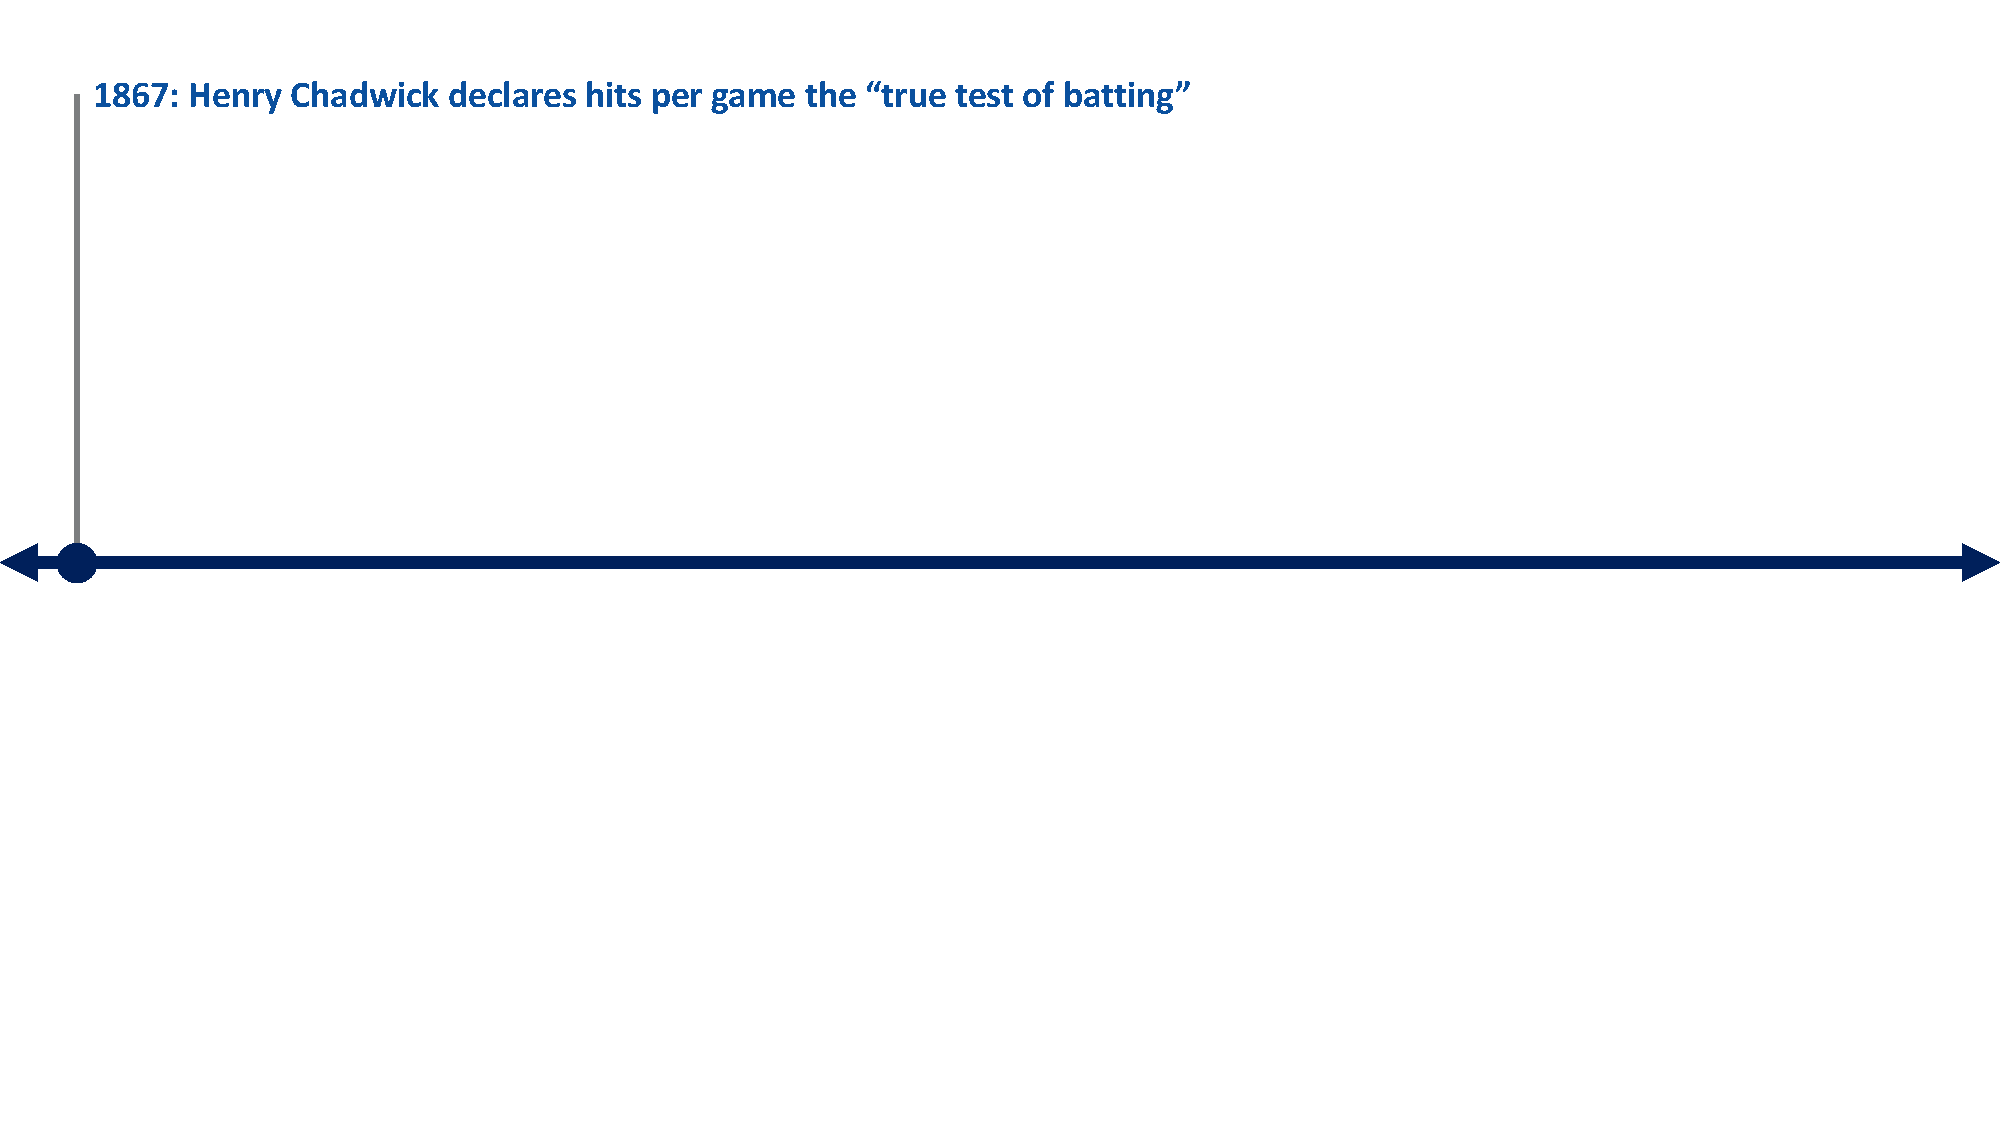
\includegraphics[width = \textwidth]{figures/timeline_1867.pdf}
\end{frame}

\begin{frame}{The Origin of Batting Average}
  \begin{columns}
    \begin{column}{0.2\textwidth}
      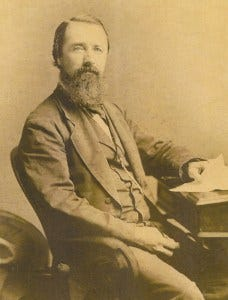
\includegraphics[width = \textwidth]{images/chadwick.jpg}
    \end{column}
    \begin{column}{0.8\textwidth}
      \begin{itemize}
        \item 1867: {\it The Ball Players' Chronicle} publishes ``The True Test of Batting'' by Henry Chadwick
        \begin{itemize}
          \item Argues for hits per game as the ``true test''
          \item Prefers hits to total bases
        \end{itemize}
      \end{itemize}
    \end{column}
  \end{columns}
  \pause
  \begin{columns}
    \begin{column}{0.8\textwidth}
      \begin{itemize}
        \item 1871: Hervie Alden Dobson writes letter to the {\it New York Clipper}
        \begin{itemize}
          \item Argues for hits per at bat over hits per game
          \item Later this came to be known as batting average
        \end{itemize}
      \end{itemize}
      $$
        \mbox{AVG} = \mbox{H} / \mbox{AB}
      $$
    \end{column}
    \begin{column}{0.2\textwidth}
      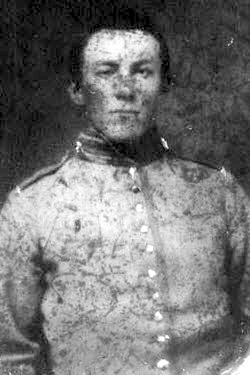
\includegraphics[width = \textwidth]{images/dobson.jpeg}
    \end{column}
  \end{columns}
  \vfill
  \hfill\color{ricegray}\tiny Source: John Thorn (2013)\\
  \hfill https://ourgame.mlblogs.com/chadwicks-choice-the-origin-of-the-batting-average-e8e9e9402d53
\end{frame}

\begin{frame}
  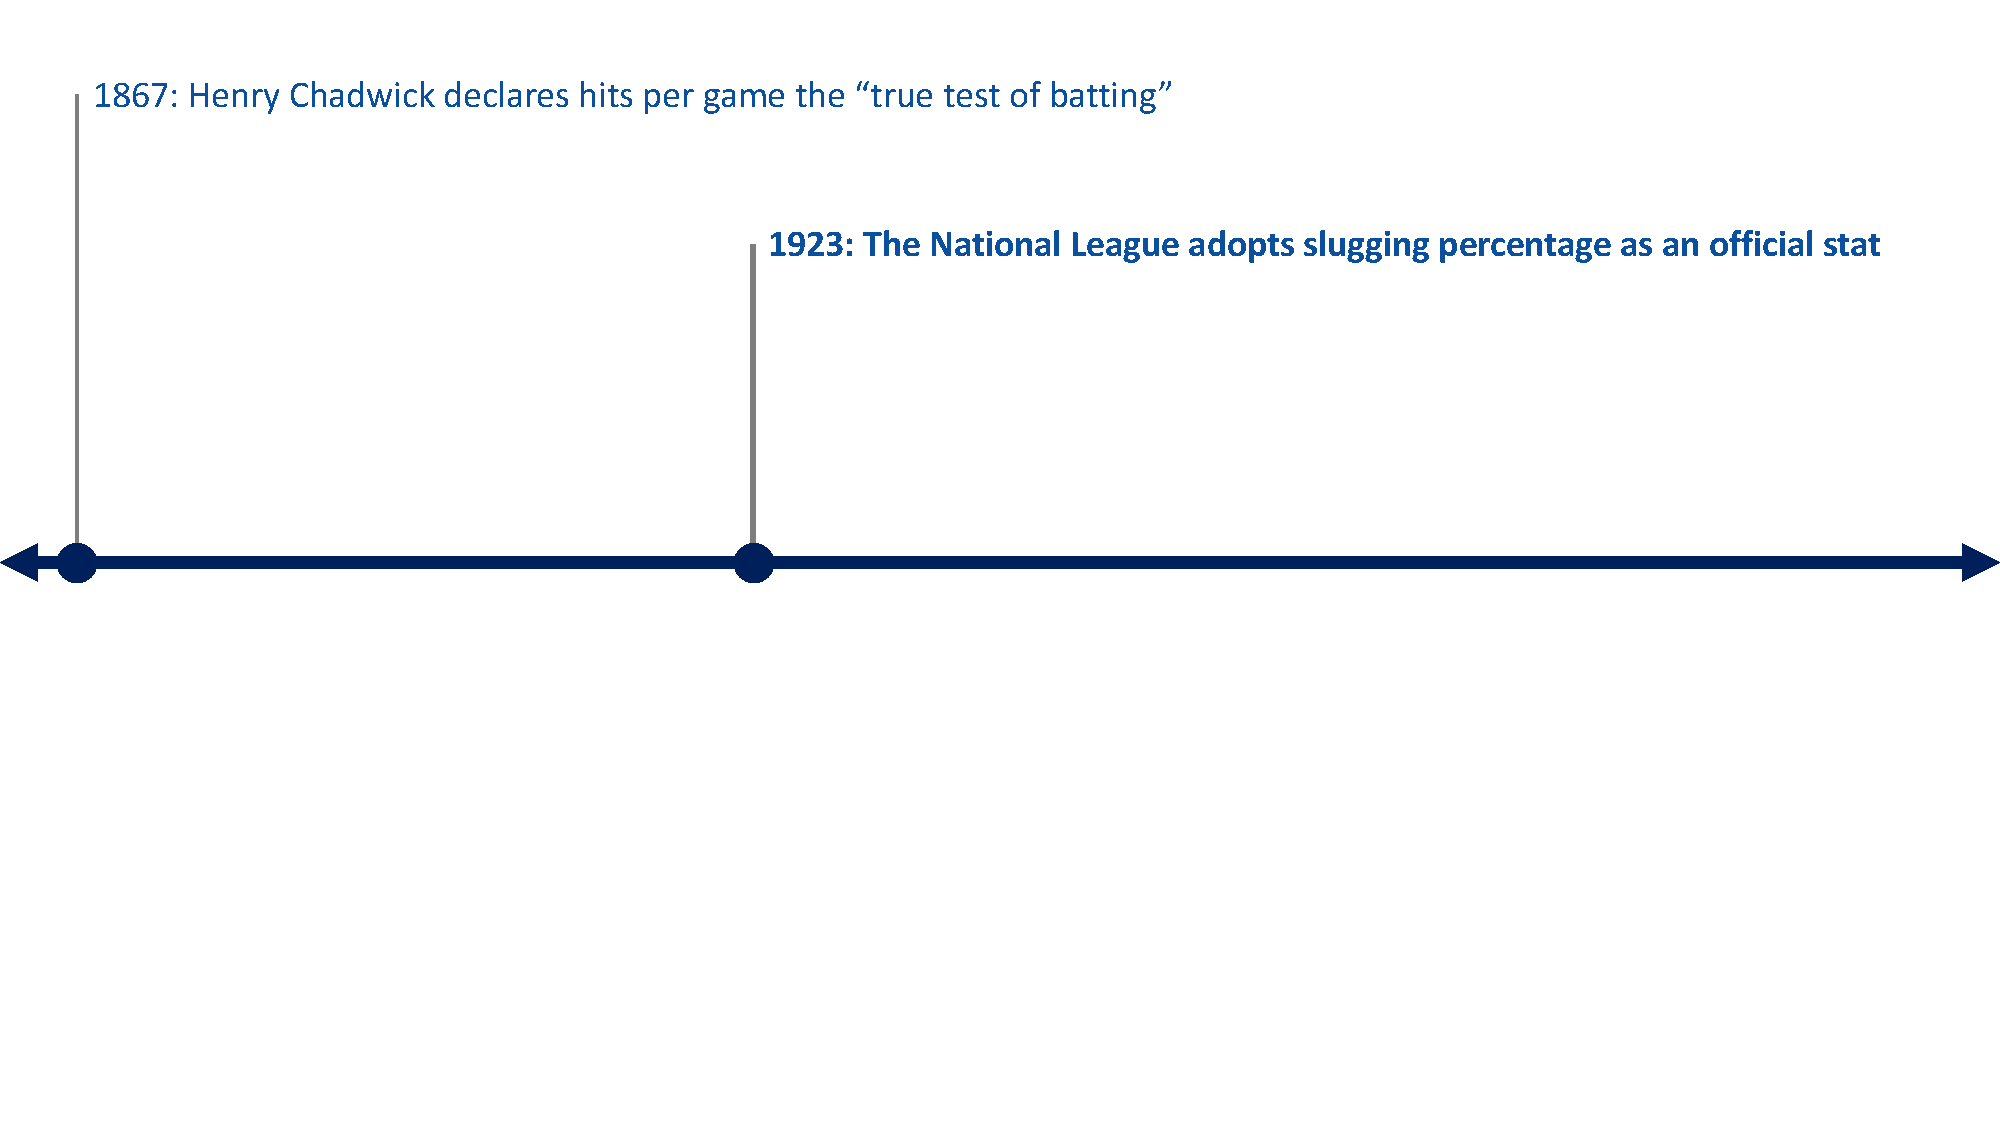
\includegraphics[width = \textwidth]{figures/timeline_1923.pdf}
\end{frame}

\begin{frame}{Slugging Percentage}
  \begin{itemize}
    \item 1923: National League adopts SLG as official stat
    \item 1946: American League adopts SLG as official stat
  \end{itemize}
  ~
  \vspace{1cm}
  ~
  $$
    \mbox{SLG}~=~\frac{\mbox{1B} + 2 \cdot \mbox{2B} + 3 \cdot \mbox{3B} + 4 \cdot \mbox{HR}}{\mbox{AB}}
  $$
\end{frame}

\begin{frame}
  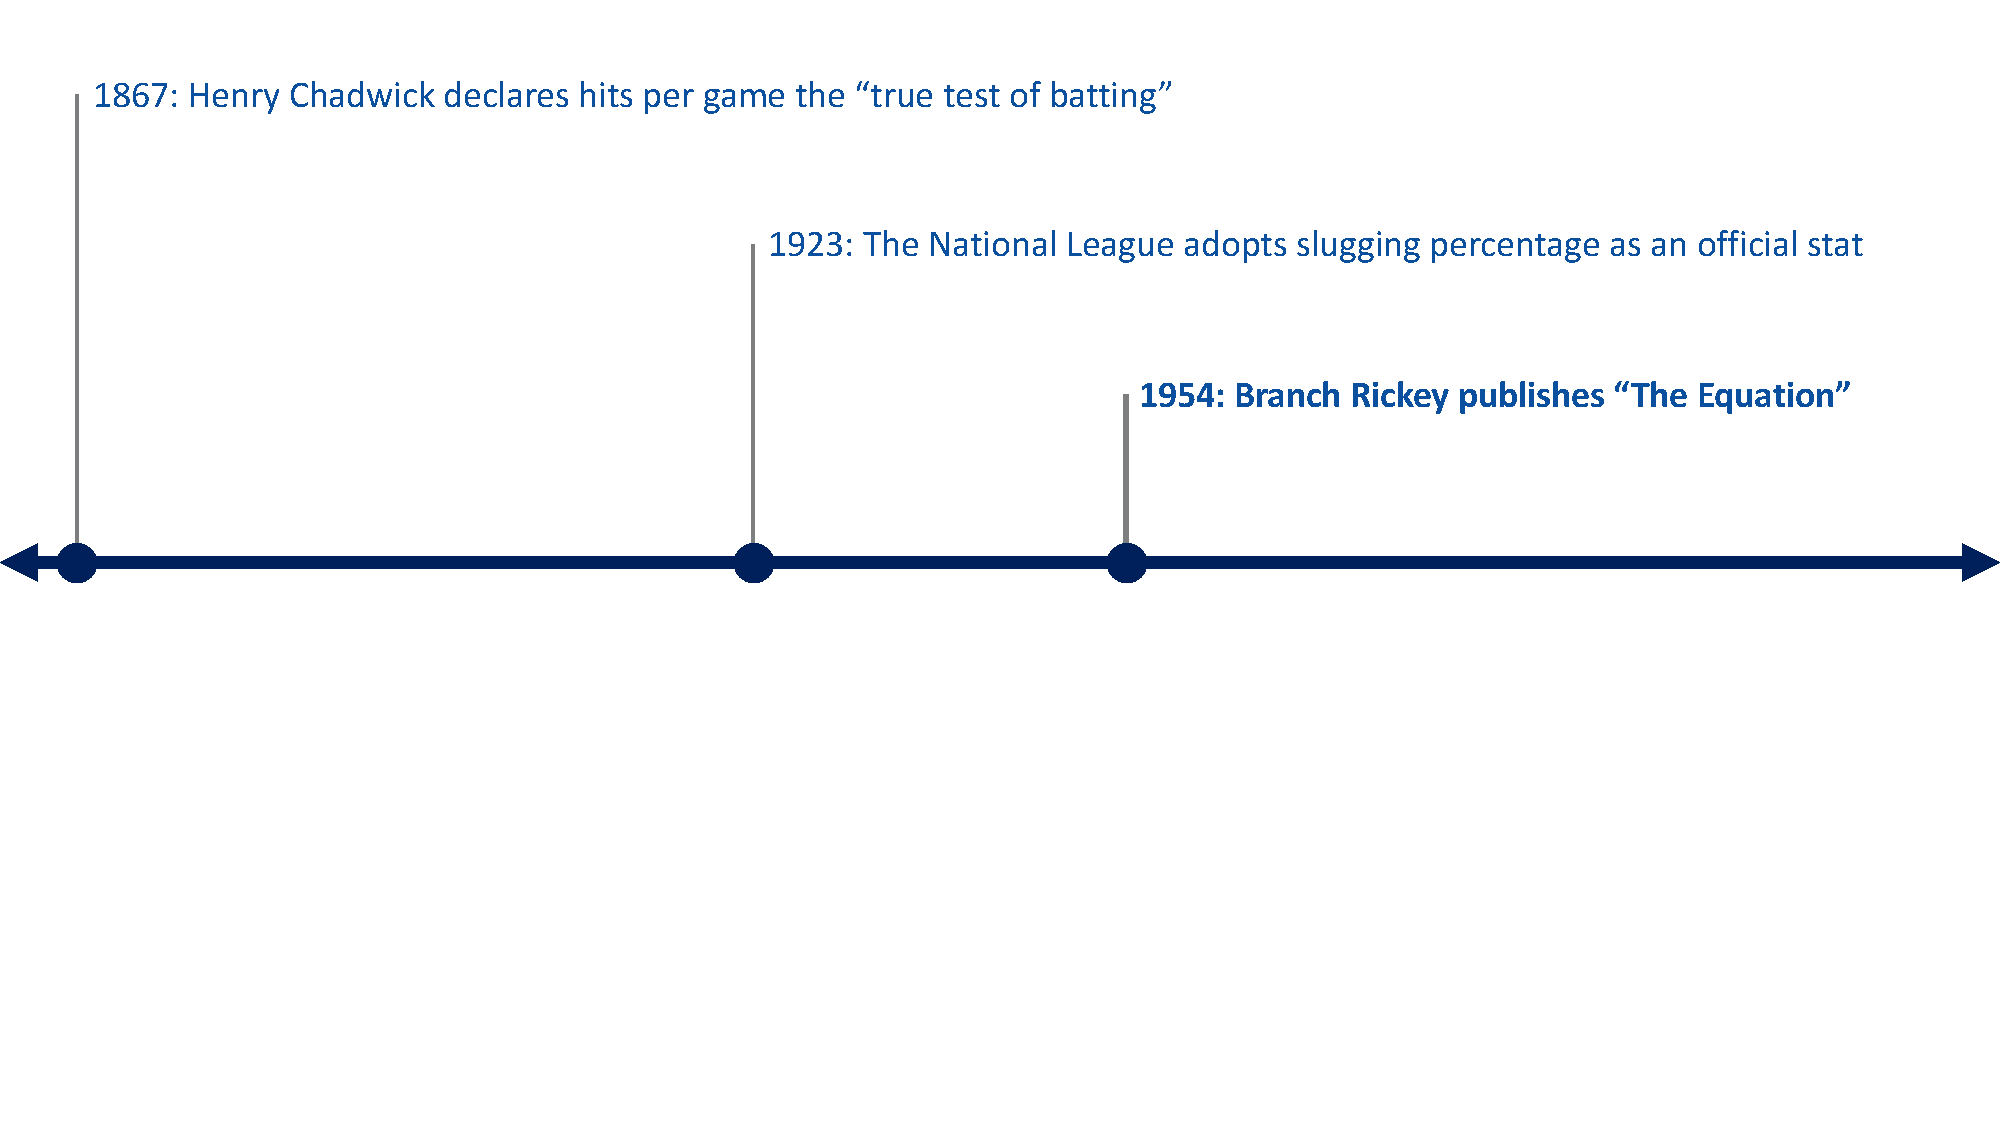
\includegraphics[width = \textwidth]{figures/timeline_1954.pdf}
\end{frame}

\begin{frame}{``The Equation''}
  \begin{itemize}
    \item 1954: Branch Rickey and Allan Roth publish ``The Equation'' in {\it Life} magazine
  \end{itemize}
  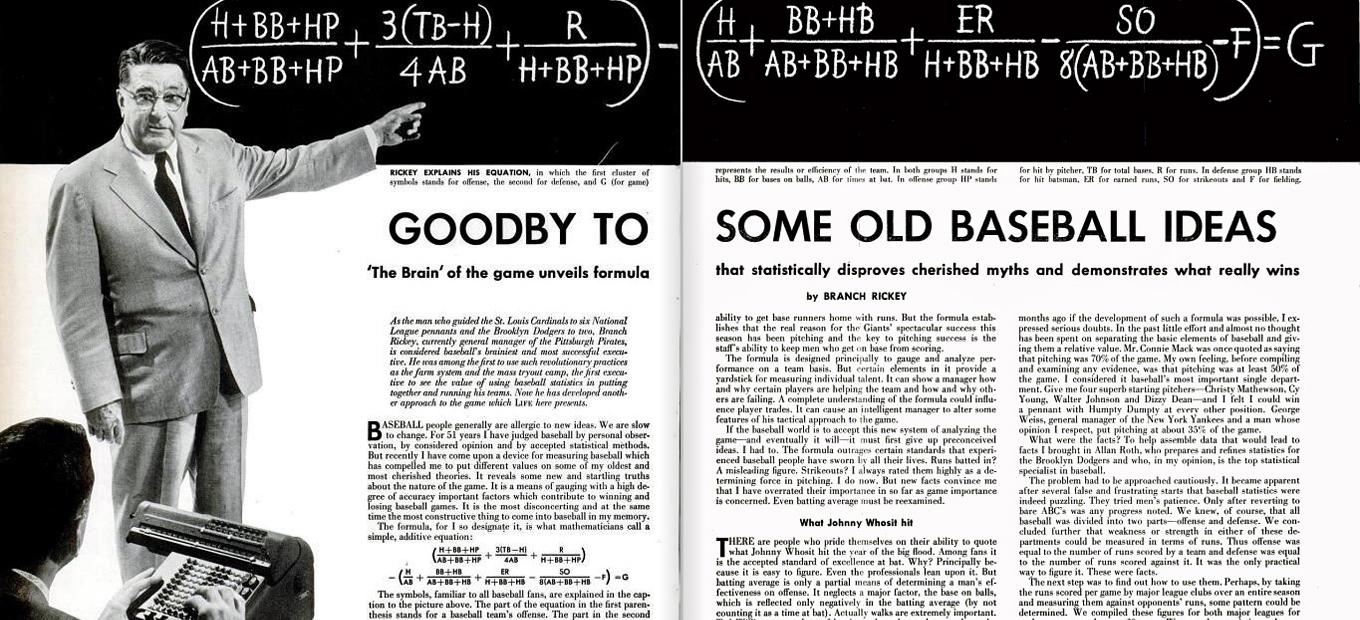
\includegraphics[width = \textwidth]{images/the_equation.jpg}
  $$
    \mbox{OBP}~=~\frac{\mbox{H} + \mbox{BB} + \mbox{HBP}}{\mbox{AB} + \mbox{BB} + \mbox{HBP} + \mbox{SF}}
  $$
\end{frame}

\begin{frame}
  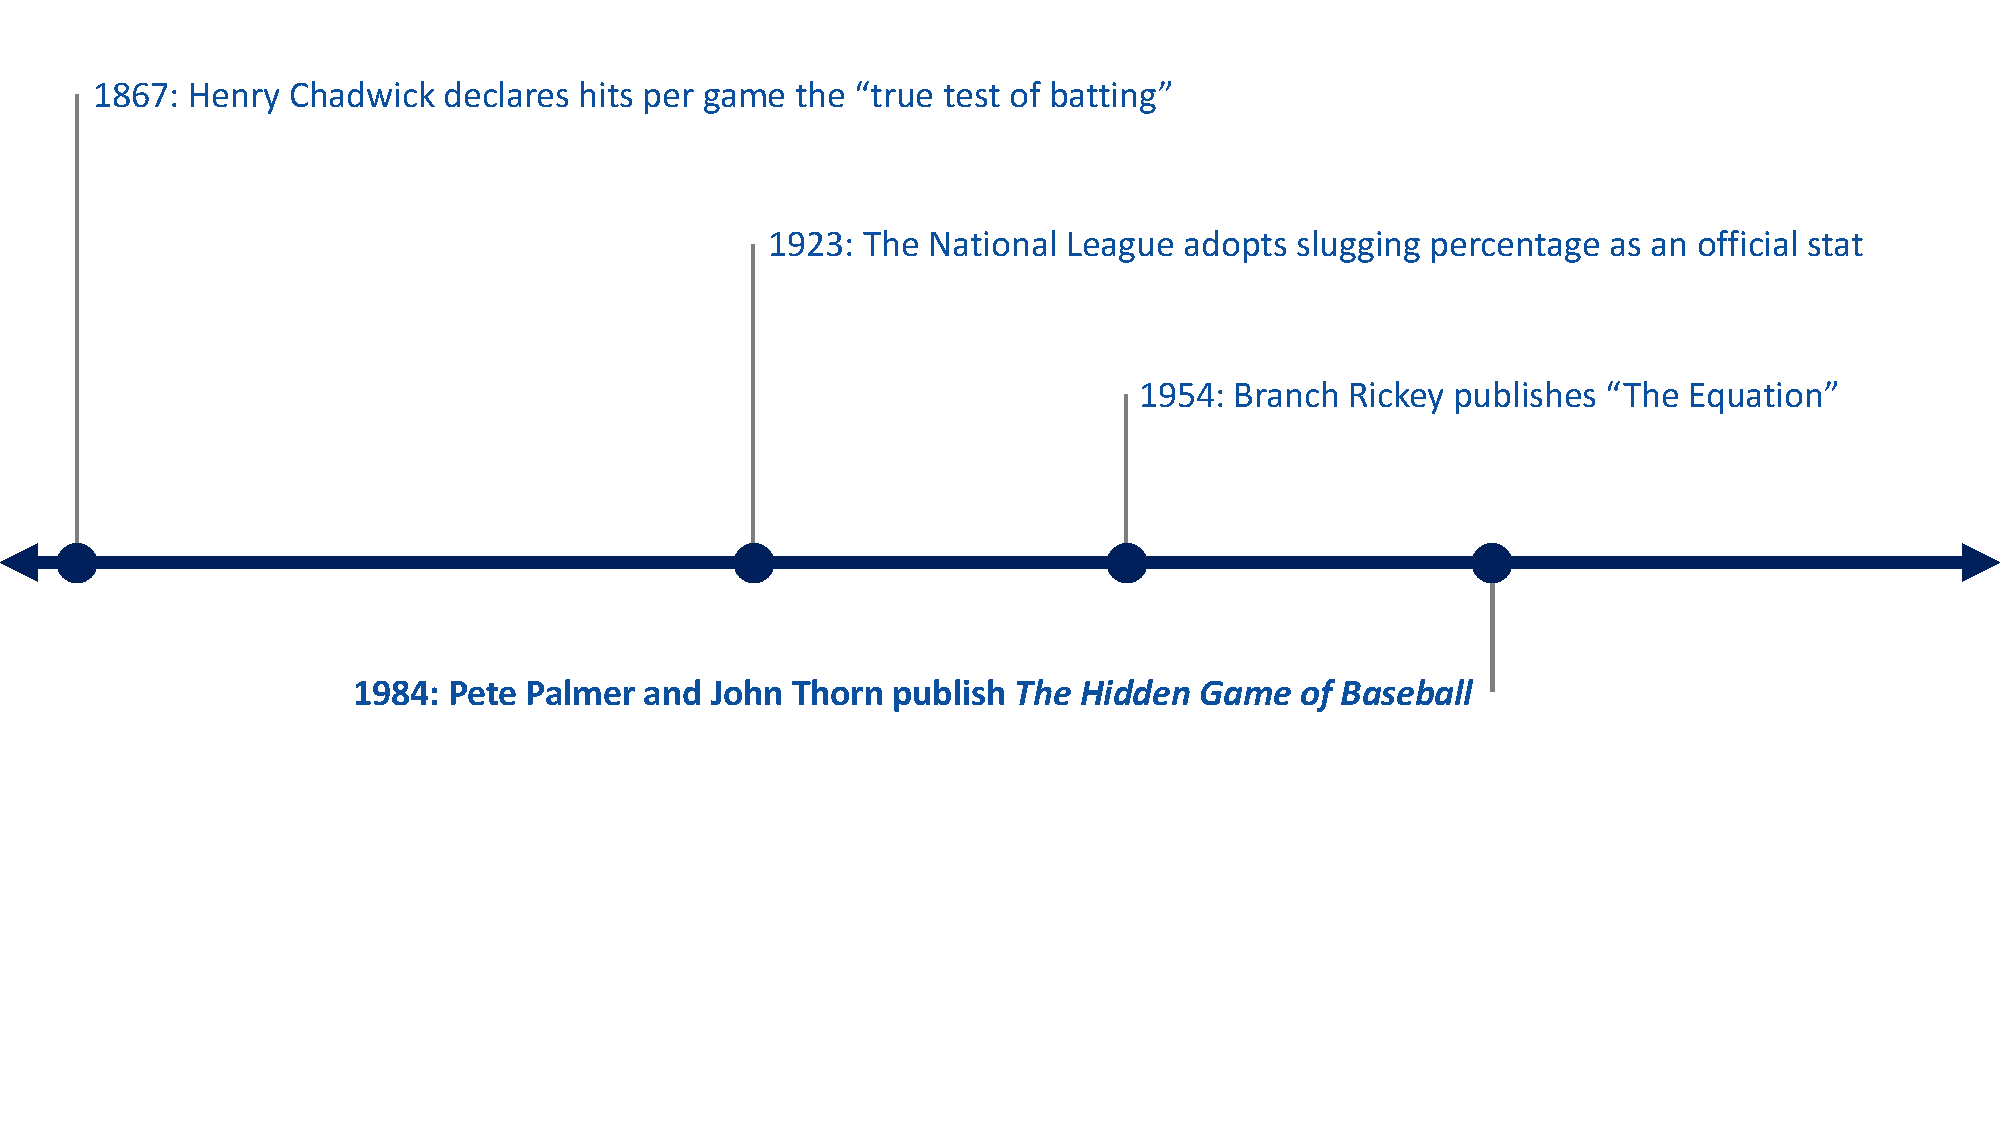
\includegraphics[width = \textwidth]{figures/timeline_1984.pdf}
\end{frame}

\begin{frame}{The Hidden Game of Baseball}
  \begin{columns}
    \begin{column}{0.3\textwidth}
      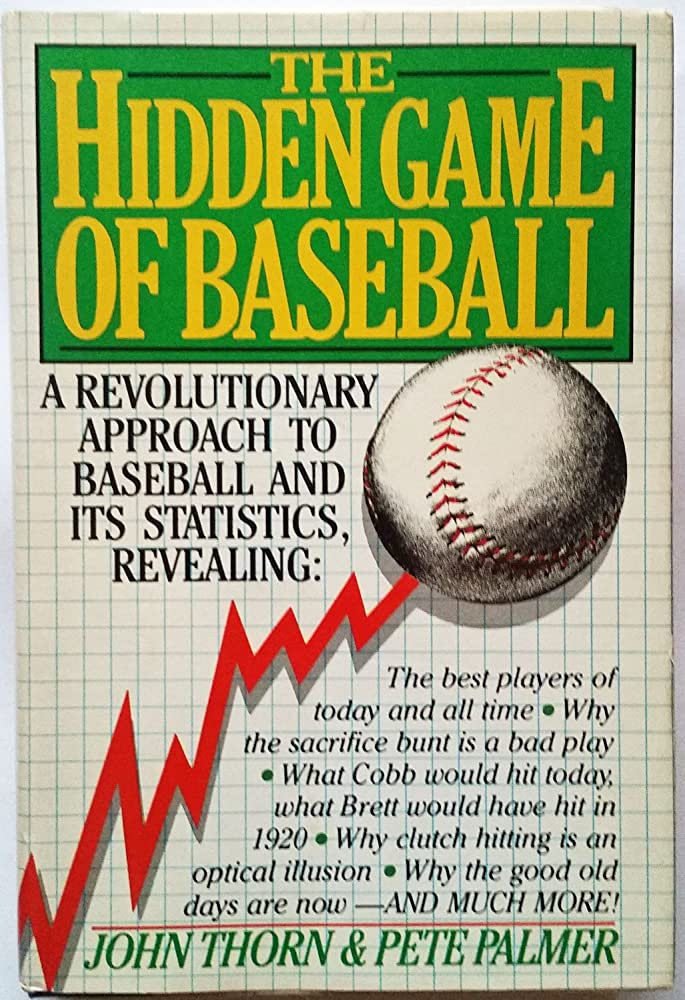
\includegraphics[width = \textwidth]{images/hidden_game.jpg}
    \end{column}
    \begin{column}{0.7\textwidth}
      \begin{itemize}
        \item 1984: John Thorn and Pete Palmer publish {\it The Hidden Game of Baseball}
        \begin{itemize}
          \item (Also in 1984: MLB adopts OBP)
        \end{itemize}
        \pause
        \item Introduces ``The Linear Weights System''
        \pause
        \item Popularizes ``On-base Plus Slugging''
      \end{itemize}
    \end{column}
  \end{columns}
  $$
    \mbox{OPS}~=~\frac{\mbox{H} + \mbox{BB} + \mbox{HBP}}{\mbox{AB} + \mbox{BB} + \mbox{HBP} + \mbox{SF}}~+~\frac{\mbox{1B} + 2 \cdot \mbox{2B} + 3 \cdot \mbox{3B} + 4 \cdot \mbox{HR}}{\mbox{AB}}
  $$
\end{frame}

\begin{frame}{A Markov model for an inning of baseball}
  \begin{itemize}
    \item Inning state: Which bases are occupied, and how many outs are there? e.g. 0-0-1-2 = runner on third base with 2 outs
    \pause
    \begin{itemize}
      \item 25 possibilities ($2 \times 2 \times 2 \times 3$ + end of inning)
    \end{itemize}
    \pause
    \item Transition probabilities from 0-0-1-2:
    \pause
    \begin{align*}
      64\% \rightarrow   ~&~ \mbox{end of inning}\\
      14\% \rightarrow   ~&~ \mbox{1-0-0-2 (+1 run)}\\
      13\% \rightarrow    ~&~ \mbox{1-0-1-2}\\
      5\% \rightarrow    ~&~ \mbox{0-1-0-2 (+1 run)}\\
      3\% \rightarrow    ~&~ \mbox{0-0-0-2 (+2 runs)}\\
      1\% \rightarrow   ~&~ \mbox{end of inning (+1 run)}\\
      <1\% \rightarrow   ~&~ \mbox{0-0-1-2 (+1 run)}
    \end{align*}
  \end{itemize}
\end{frame}

\begin{frame}{Transition probability matrix}
  \begin{itemize}
    \item $A \in [0, 1]^{25\times25}$ encodes transition probabilities between states
    \item $A_{ij}$ is the probability of transitioning to state $j$ from state $i$
    \pause
    \item Multiply $A$ by itself to get multi-step transition probability
    \begin{itemize}
      \item $A^2$ is transition probability matrix after 2 steps
      \item $A^3$ is transition probability matrix after 3 steps
      \item ...
      \item $A^\infty$ gives terminal state probability\\
      {\it All initial states converge to end of inning}
    \end{itemize}
  \end{itemize}
  \pause
  \vfill
  Exercise: How can we use this model to calculate the expected number of runs scored from each initial state?
\end{frame}

\begin{frame}{(My) Solution}
  \begin{itemize}
    \item Track runs scored in the inning state! e.g. 0-0-1-2-$X$ =\\
      runner on third base with 2 outs, $X$ runs have scored
    \pause
    \item Infinite possibilities!
    \pause
    \item But can safely ignore $X > 9$ (very small probability)
    \pause
    \begin{itemize}
      \item 250 possibilities (25 from earlier $\times$ 10 values of $X$)
      \item $A \in [0, 1]^{250\times250}$ encodes transition probabilities
      \item $A^{20}$ is close enough to $A^\infty$
    \end{itemize}
  \end{itemize}
\end{frame}

\begin{frame}{Run Expectancy by Base-Out State}
  \begin{columns}
    \begin{column}{0.3\textwidth}
      \centering
      \begin{tabular}{c|c}
        State   & RE\\
        \hline
        1-1-1-0 & 2.41\\
        ... & ...\\
        0-1-0-0 & 1.15\\
        ... & ...\\
        1-0-0-0 & 0.91\\
        ... & ...\\
        0-0-0-0 & 0.51\\
        ... & ...\\
        0-0-0-1 & 0.27\\
        ... & ...\\
        0-0-0-2 & 0.11\\
        0-0-0-3 & 0.00\\
      \end{tabular}
    \end{column}
    \begin{column}{0.7\textwidth}
      \footnotesize
      \pause
      Example \#1: Leadoff double
      \begin{align*}
        \mbox{RE(0-1-0-0)} - \mbox{RE(0-0-0-0)} &= 1.15 - 0.51\\
                                                &= +0.64 \mbox{ runs!}
      \end{align*}
      ~\\
      \pause
      Example \#2: Bases empty, two-out double
      \begin{align*}
        \mbox{\color{ricegray} RE(0-1-0-2)} - \mbox{RE(0-0-0-2)} &= \mbox{\color{ricegray} 0.33} - 0.11\\
                                                                 &= +0.22 \mbox{ runs!}
      \end{align*}
      ~\\
      \pause
      Example \#3: Bases loaded, no-out double
      \begin{align*}
        3 + \mbox{RE(0-1-0-0)} - \mbox{RE(1-1-1-0)} &= 3 + 1.15 - 2.41\\
                                                    &= +1.74 \mbox{ runs!}
      \end{align*}
    \end{column}
  \end{columns}
\end{frame}

%\begin{frame}{Average Change in Run Expectancy by Event}
%  \begin{tabular}{c|c}
%    Event         & Change in RE\\
%    \hline
%    Home Run      & $+1.38$     \\
%    Triple        & $+1.06$     \\
%    Double        & $+0.76$     \\
%    Single        & $+0.46$     \\
%    Hit By Pitch  & $+0.35$     \\
%    Walk          & $+0.33$     \\
%    Flyout        & $-0.27$     \\
%    Strikeout     & $-0.27$     \\
%    Groundout     & $-0.29$     \\
%  \end{tabular}
%\end{frame}
%
%\begin{frame}{Average Change in Run Expectancy by Event}
%  \begin{tabular}{c|cc}
%    Event         & Change in RE  & {\it vs} Out\\
%    \hline
%    Home Run      & $+1.38$       & 1.65\\
%    Triple        & $+1.06$       & 1.33\\
%    Double        & $+0.76$       & 1.03\\
%    Single        & $+0.46$       & 0.73\\
%    Hit By Pitch  & $+0.35$       & 0.62\\
%    Walk          & $+0.33$       & 0.60\\
%    Flyout        & $-0.27$       & --- \\
%    Strikeout     & $-0.27$       & --- \\
%    Groundout     & $-0.29$       & --- \\
%  \end{tabular}
%\end{frame}

\begin{frame}{Average Change in Run Expectancy by Event}
  \begin{tabular}{c|ccc}
    Event         & Change in RE  & {\it vs} Out & OPS Weight\\
    \hline
    Home Run      & $+1.38$       & 1.65    & 5\\
    Triple        & $+1.06$       & 1.33    & 4\\
    Double        & $+0.76$       & 1.03    & 3\\
    Single        & $+0.46$       & 0.73    & 2\\
    Hit By Pitch  & $+0.35$       & 0.62    & 1\\
    Walk          & $+0.33$       & 0.60    & 1\\
    Flyout        & $-0.27$       & ---     & 0\\
    Strikeout     & $-0.27$       & ---     & 0\\
    Groundout     & $-0.29$       & ---     & 0\\
  \end{tabular}
\end{frame}

\begin{frame}{Takeaway \#1}
  Sport analytics is less {\it crafting} metrics and more {\it deriving} them.
\end{frame}

\begin{frame}{Two Perspectives}
  \centering
  \footnotesize
  \begin{tabular}{c|ccl|cc}
    Player  & Start State & Event     & End State     & RE24    & LW\\
    \hline
            & 0-0-0-2     & Groundout & End of Inning & $-0.11$ & $-0.29$\\
            & 1-0-0-0     & Strikeout & 1-0-0-1       & $-0.38$ & $-0.27$\\
    A       & 0-1-1-1     & Flyout    & 0-1-0-2 (+1)  & $-0.07$ & $-0.27$\\
            & 0-1-1-2     & Single    & 1-0-0-2 (+2)  & $+1.63$ & $+0.46$\\
      & \multicolumn{3}{r|}{\color{ricegray} Total} & \color{ricegray} $+1.07$ & \color{ricegray} $-0.37$\\
    \hline
            & 0-0-0-2     & Single    & 1-0-0-2       & $+0.12$ & $+0.46$\\
            & 1-0-0-0     & Groundout & 0-0-0-2       & $-0.81$ & $-0.29$\\
    B       & 0-1-1-1     & Strikeout & 0-1-1-2       & $-0.80$ & $-0.27$\\
            & 0-1-1-2     & Flyout    & End of Inning & $-0.60$ & $-0.27$\\
      & \multicolumn{3}{r|}{\color{ricegray} Total} & \color{ricegray} $-2.09$ & \color{ricegray} $-0.37$\\
  \end{tabular}
\end{frame}

%\begin{frame}{LW vs. RE24}
%  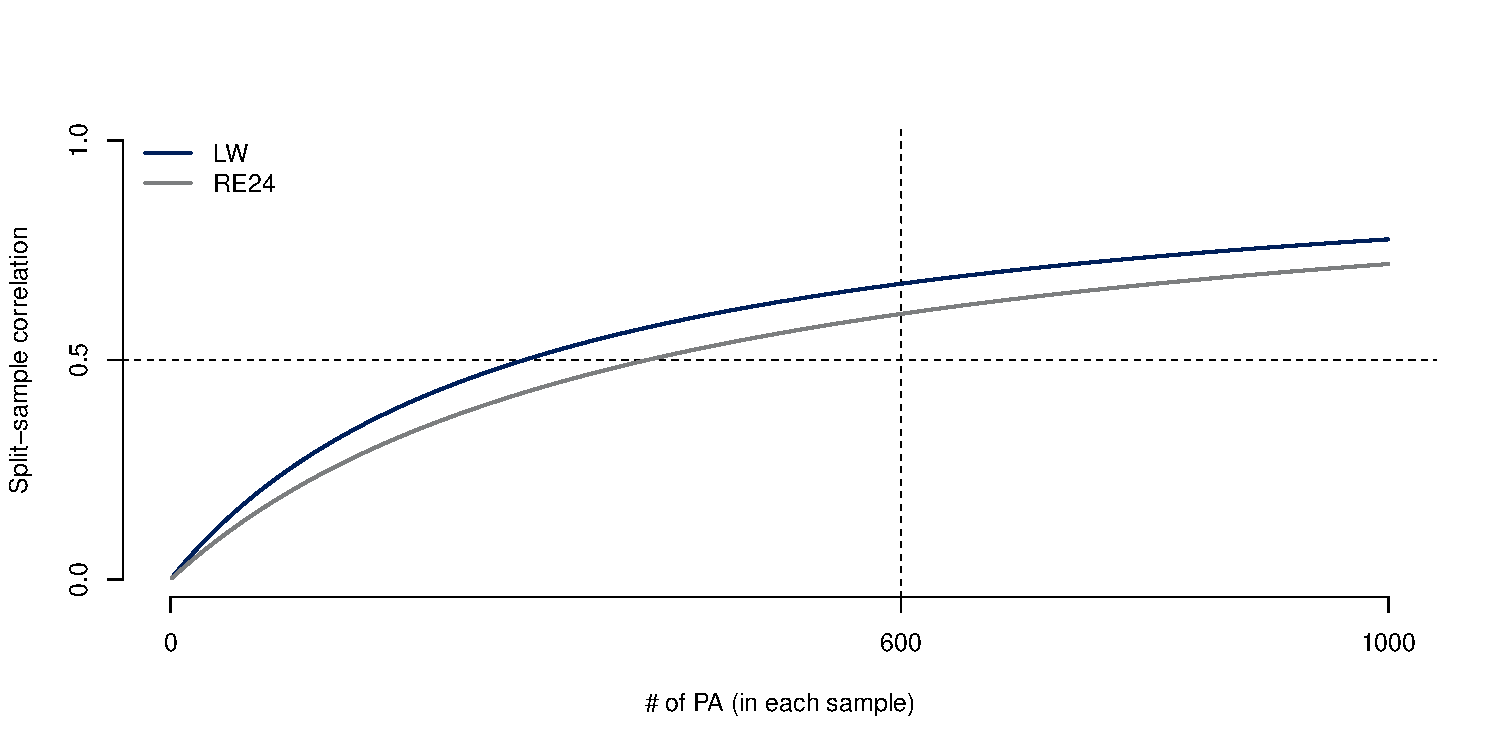
\includegraphics[width = \textwidth]{figures/re24_lw.pdf}
%\end{frame}

\begin{frame}{LW vs. RE24}
  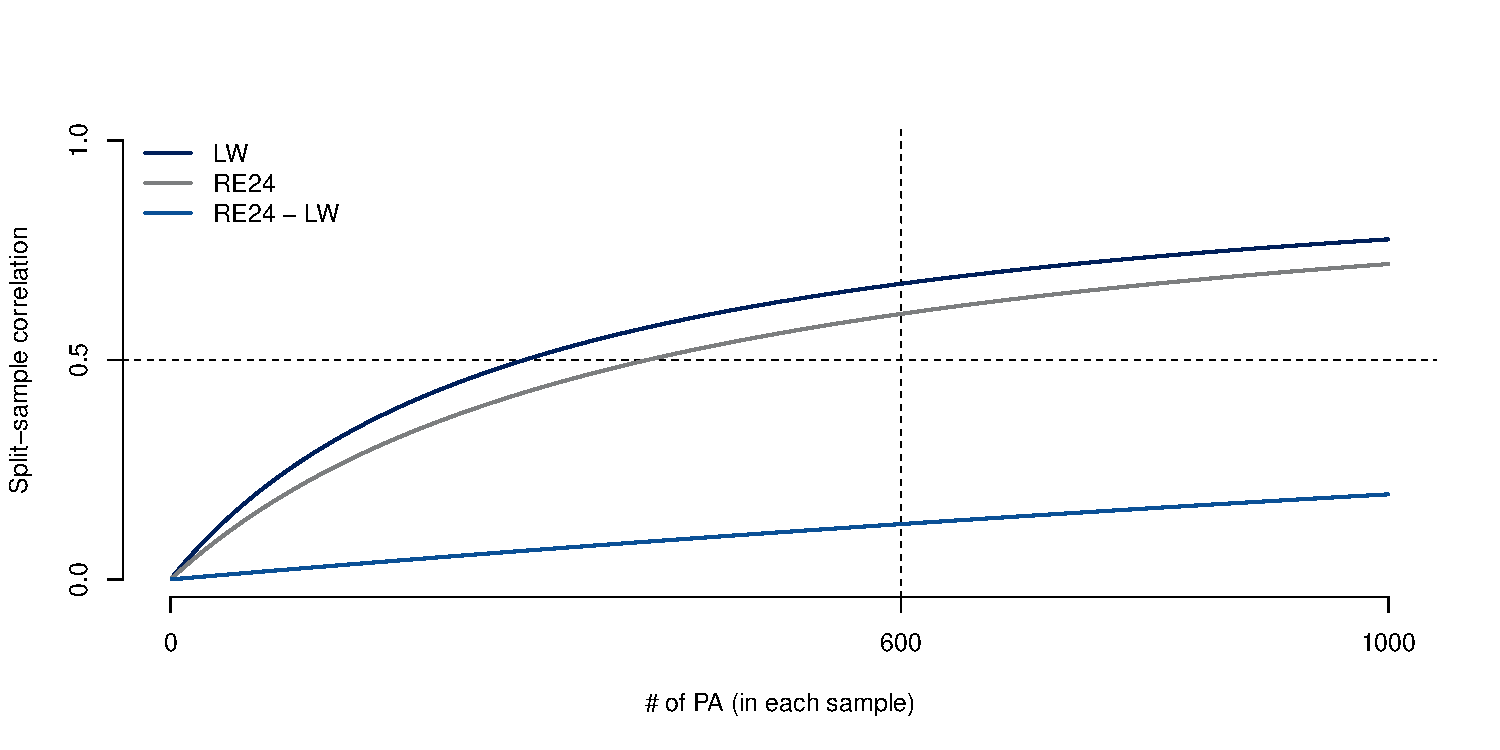
\includegraphics[width = \textwidth]{figures/re24_lw_diff.pdf}
\end{frame}

\begin{frame}
  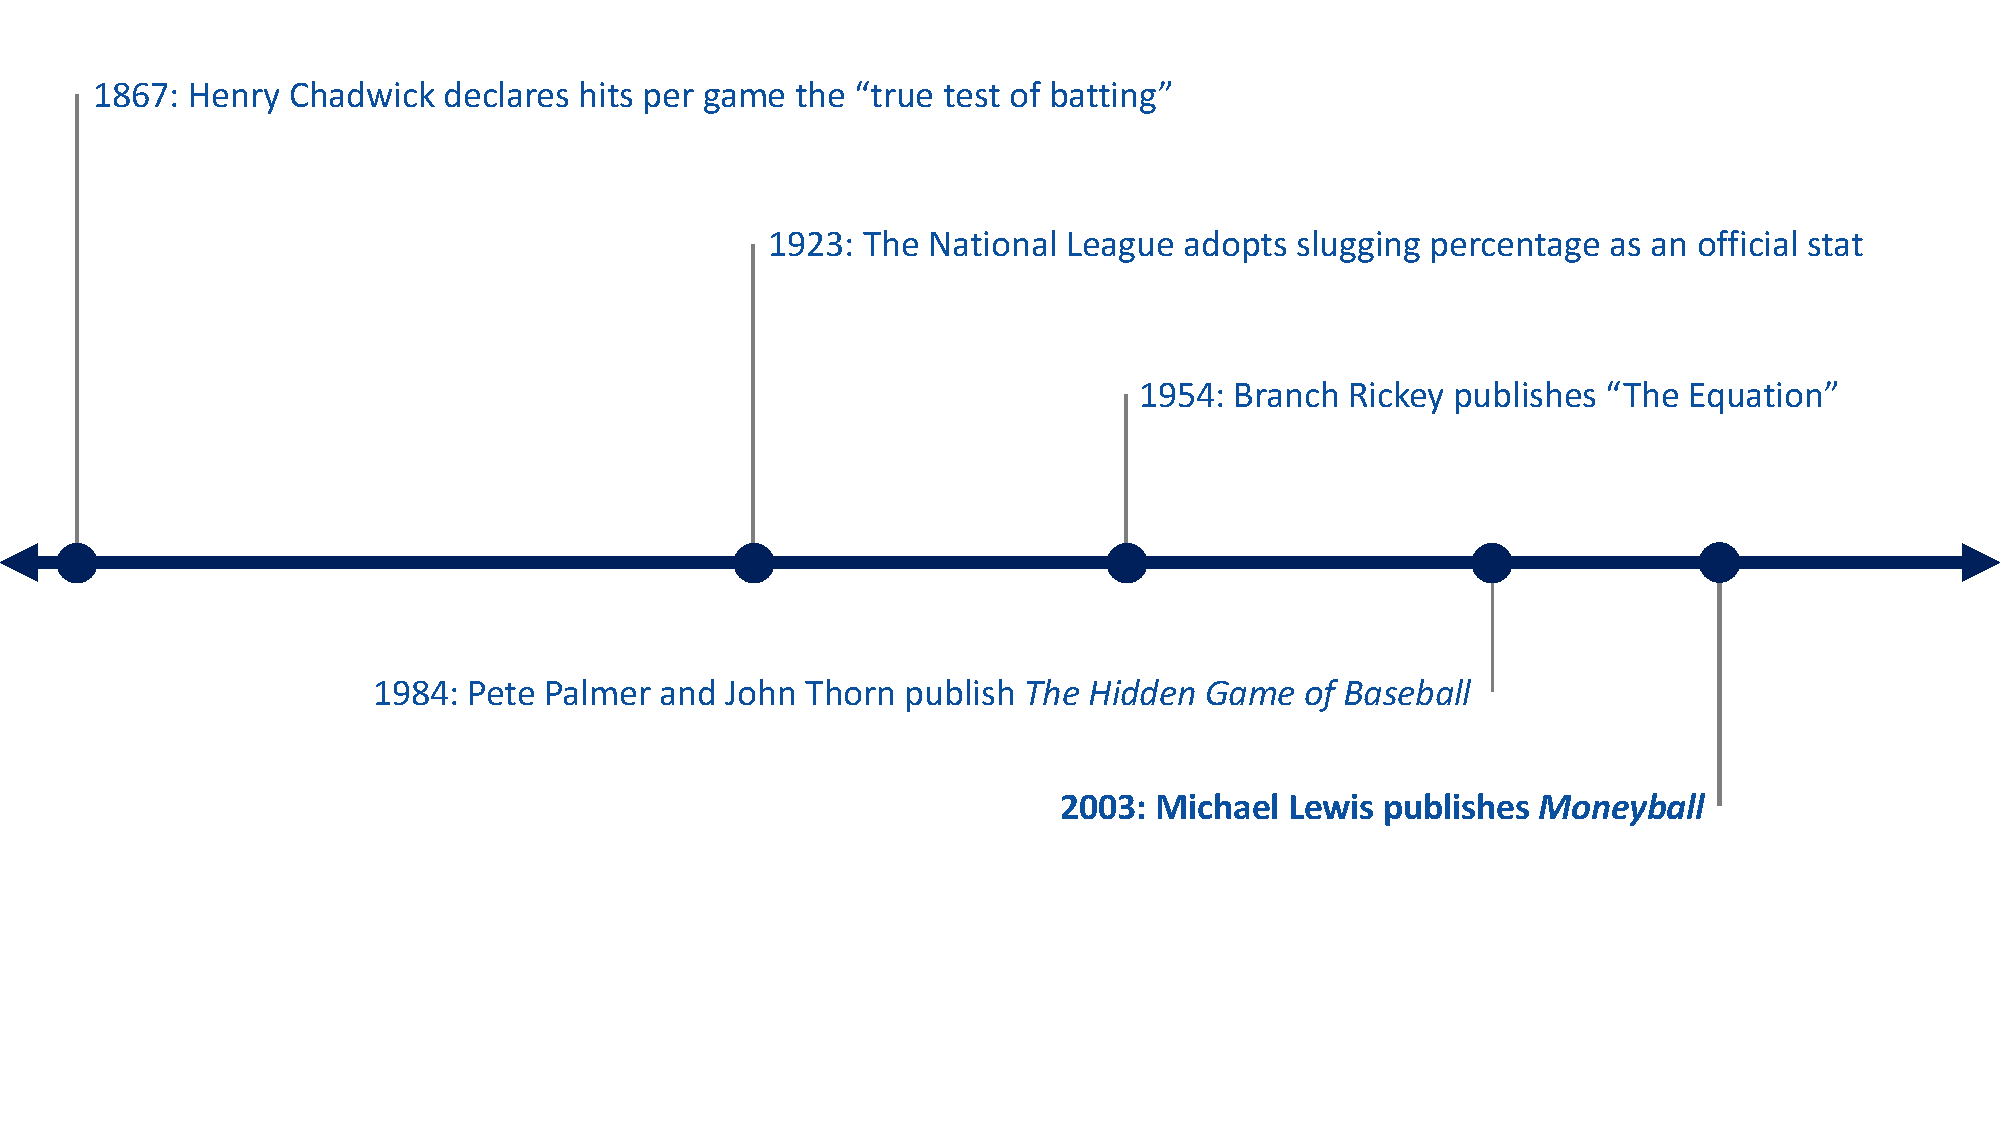
\includegraphics[width = \textwidth]{figures/timeline_2003.pdf}
\end{frame}

\begin{frame}{Moneyball, and OBP vs. AVG}
  \begin{columns}
    \begin{column}{0.3\textwidth}
      \centering
      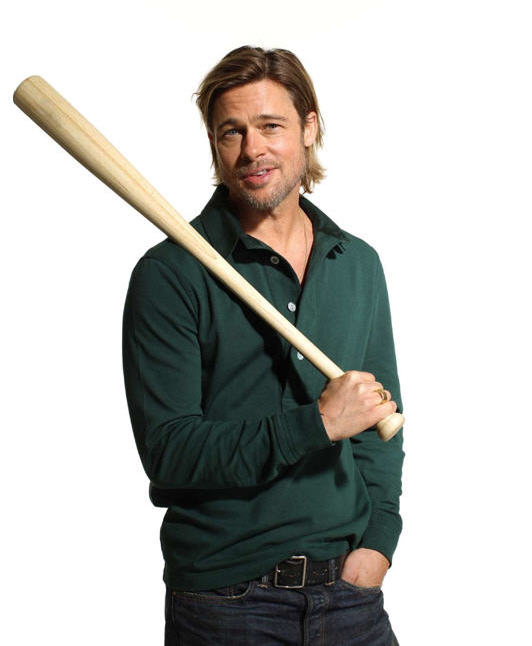
\includegraphics[width = \textwidth]{images/brad_pitt.jpg}\\
      \tiny \color{ricegray} \it Sports Illustrated
    \end{column}
    \begin{column}{0.7\textwidth}
      \begin{itemize}
        \item 2003: Michael Lewis publishes {\it Moneyball}
        \item Why was batting average favored over on-base percentage for so long?
        \item Two criteria: Does it correlate to team success? Is it reliable?
        \begin{itemize}
          \item Correlation with team success:\\ see previous slides
          \item Reliability: Less obvious
        \end{itemize}
      \end{itemize}
    \end{column}
  \end{columns}
\end{frame}

\begin{frame}{OBP vs. AVG}
  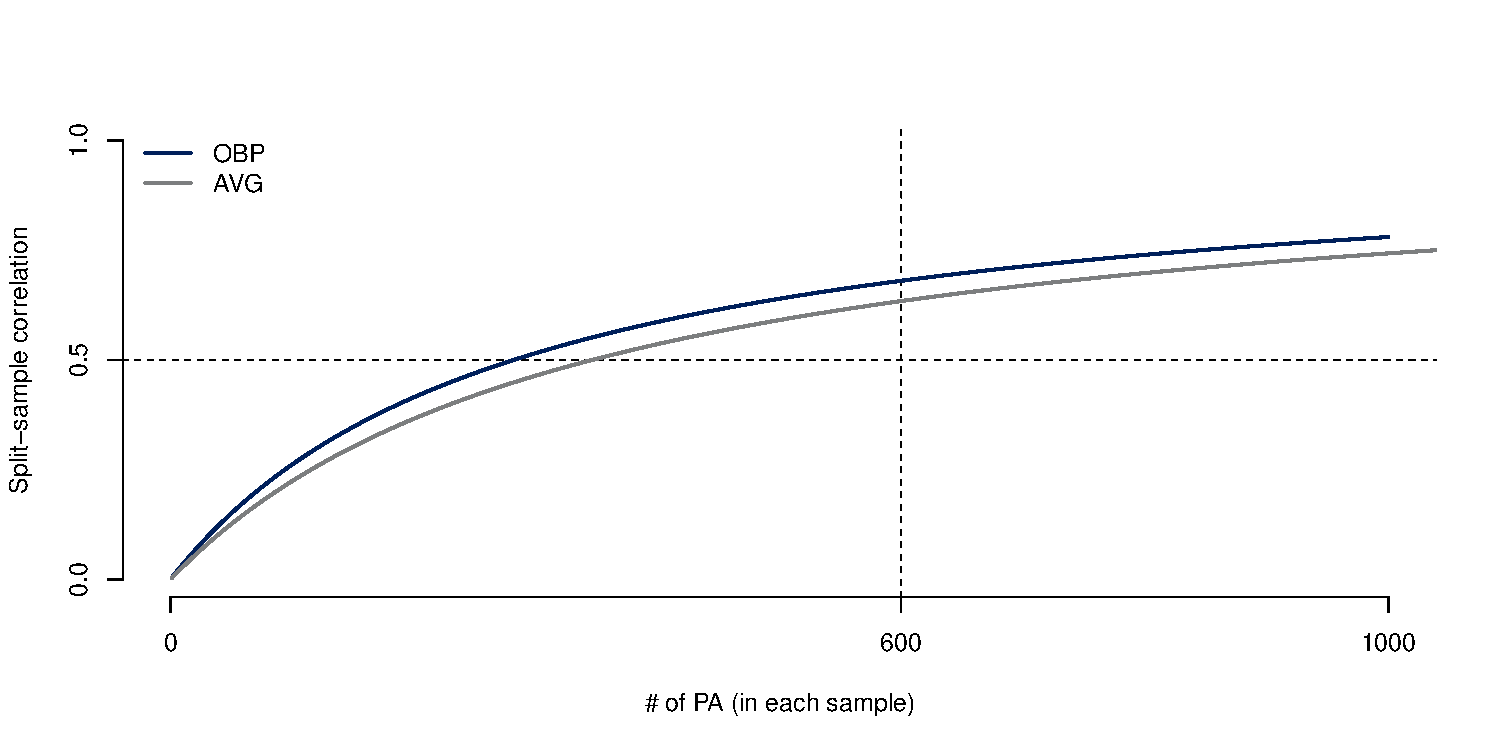
\includegraphics[width = \textwidth]{figures/avg_obp.pdf}
\end{frame}

\begin{frame}
  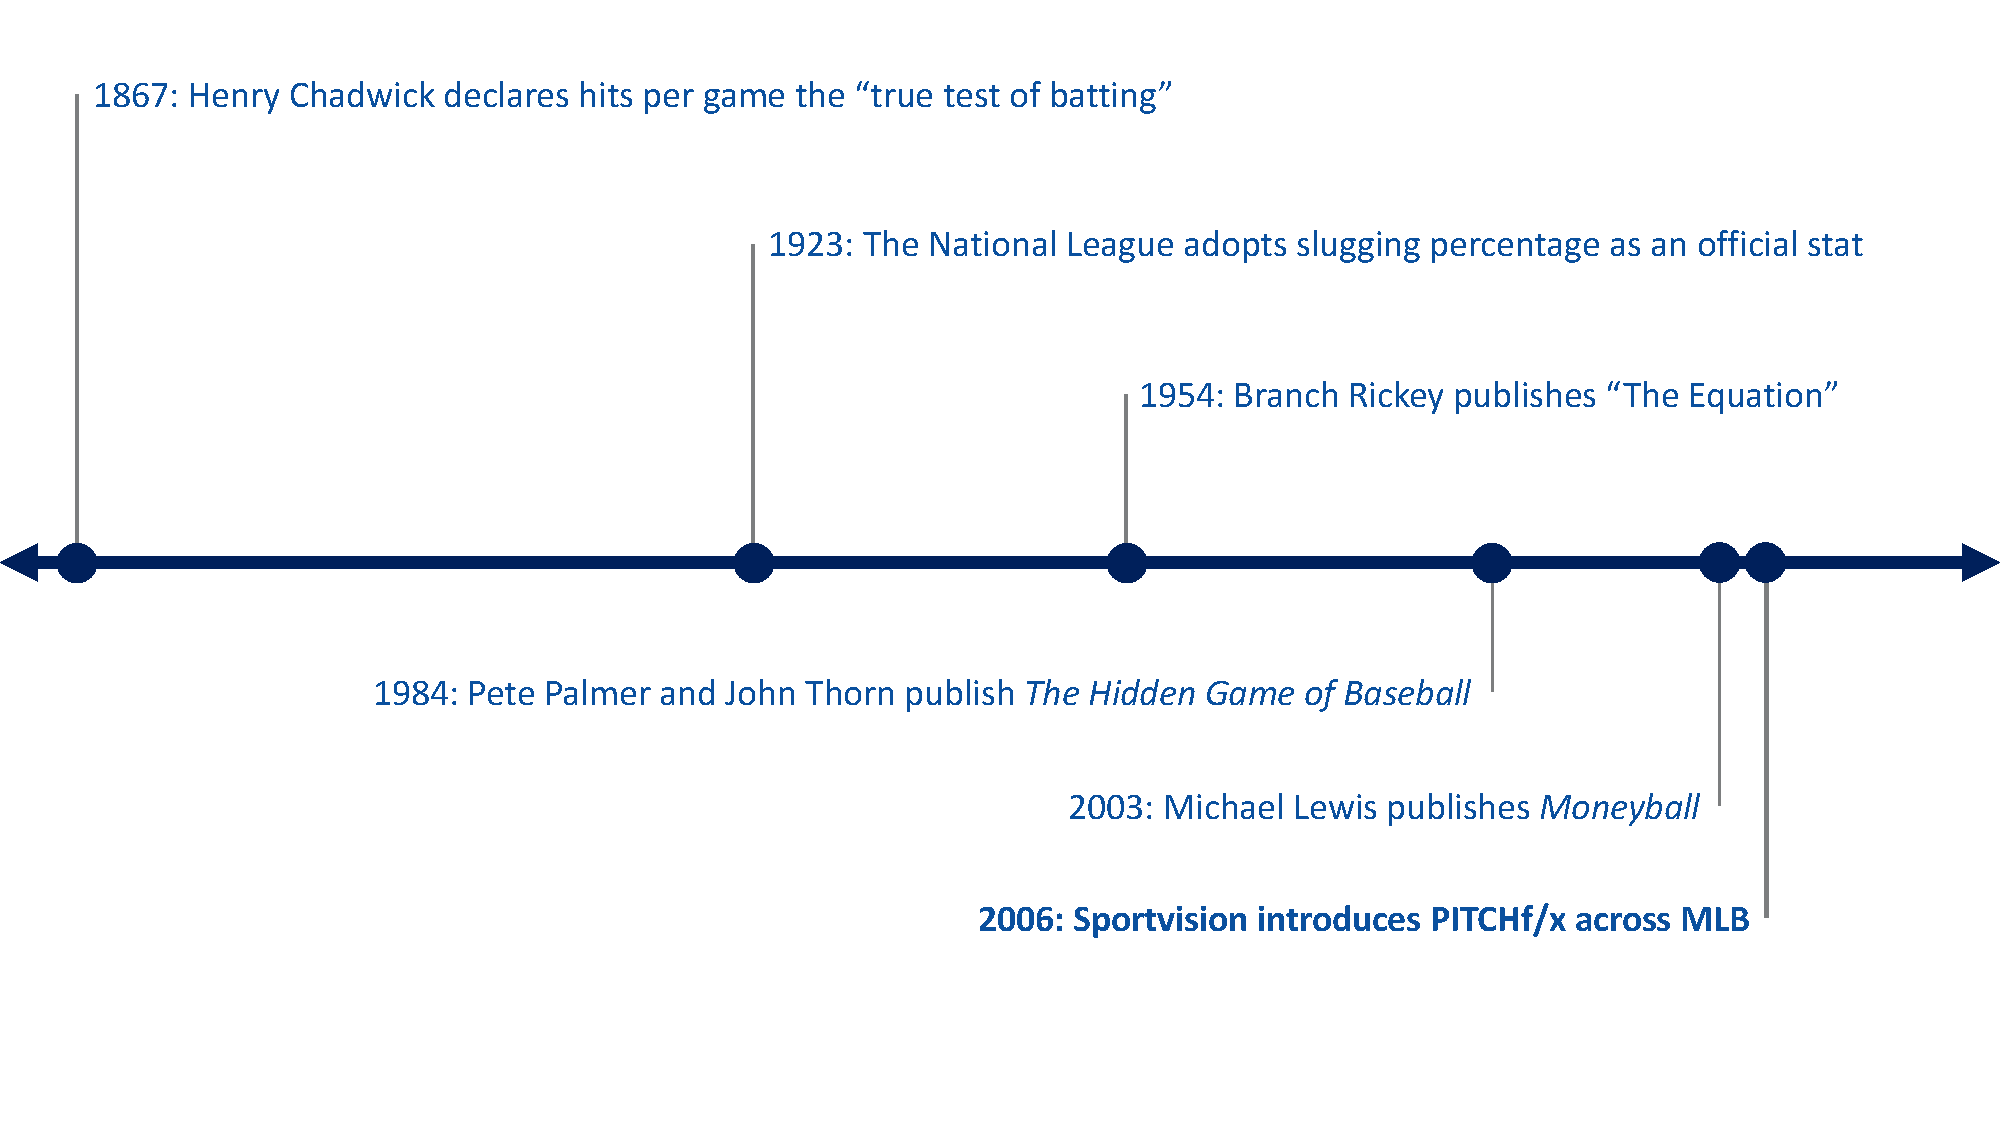
\includegraphics[width = \textwidth]{figures/timeline_2006.pdf}
\end{frame}

\begin{frame}{Ball Tracking}
  \begin{columns}
    \begin{column}{0.6\textwidth}
      \begin{itemize}
        \item 2006: Sportvision introduces PITCHf/x across MLB
        \item 2009: Sportvision introduces HITf/x across MLB
        \begin{itemize}
          \item Based on computer vision
        \end{itemize}
        ~\\
        \item 2017: TrackMan replaces Sportvision pitch and hit tracking
        \begin{itemize}
          \item Based on Doppler radar
        \end{itemize}
      \end{itemize}
    \end{column}
    \pause
    \begin{column}{0.4\textwidth}
      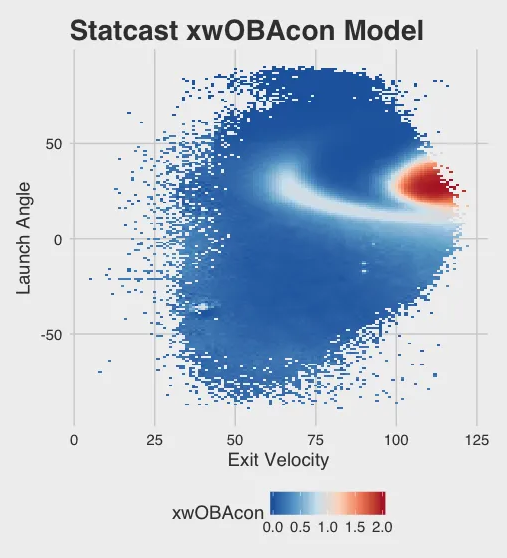
\includegraphics[width = \textwidth]{images/xwobacon.png}
    \end{column}
  \end{columns}
\end{frame}

%\begin{frame}{A Third Perspective}
%  \footnotesize
%  \begin{tabular}{c|cccc|cc}
%    Player  & Start State & Event     & \color{ricerichblue} EV  & \color{ricerichblue} LA   & RE24    & LW     \\
%    \hline
%            & 0-0-0-2     & Groundout & \color{ricerichblue} 80  & \color{ricerichblue} -20  & $-0.11$ & $-0.29$\\
%            & 1-0-0-0     & Strikeout &                          & \color{ricerichblue}      & $-0.38$ & $-0.27$\\
%    A       & 0-1-1-1     & Flyout    & \color{ricerichblue} 93  & \color{ricerichblue}  32  & $-0.07$ & $-0.27$\\
%            & 0-1-1-2     & Single    & \color{ricerichblue} 87  & \color{ricerichblue}  -2  & $+1.63$ & $+0.46$\\
%      & \multicolumn{4}{r|}{\color{ricegray} Total} & \color{ricegray} $+1.07$ & \color{ricegray} $-0.37$\\
%    \hline
%            & 0-0-0-2     & Single    & \color{ricerichblue} 91  & \color{ricerichblue}  16  & $+0.12$ & $+0.46$\\
%            & 1-0-0-0     & Groundout & \color{ricerichblue} 96  & \color{ricerichblue} -12  & $-0.81$ & $-0.29$\\
%    B       & 0-1-1-1     & Strikeout &                          & \color{ricerichblue}      & $-0.80$ & $-0.27$\\
%            & 0-1-1-2     & Flyout    & \color{ricerichblue} 90  & \color{ricerichblue}  24  & $-0.60$ & $-0.27$\\
%      & \multicolumn{4}{r|}{\color{ricegray} Total} & \color{ricegray} $-2.09$ & \color{ricegray} $-0.37$\\
%  \end{tabular}
%\end{frame}

\begin{frame}{A Third Perspective}
  \footnotesize
  \begin{tabular}{c|cccc|ccc}
    Player  & Start State & Event     & \color{ricerichblue} EV  & \color{ricerichblue} LA   & RE24    & LW      & \color{ricerichblue} xLW\\
    \hline
            & 0-0-0-2     & Groundout & \color{ricerichblue} 80  & \color{ricerichblue} -20  & $-0.11$ & $-0.29$ & \color{ricerichblue} $-0.22$\\
            & 1-0-0-0     & Strikeout &                          & \color{ricerichblue}      & $-0.38$ & $-0.27$ & \color{ricerichblue} $-0.27$\\
    A       & 0-1-1-1     & Flyout    & \color{ricerichblue} 93  & \color{ricerichblue}  32  & $-0.07$ & $-0.27$ & \color{ricerichblue} $-0.10$\\
            & 0-1-1-2     & Single    & \color{ricerichblue} 87  & \color{ricerichblue}  -2  & $+1.63$ & $+0.46$ & \color{ricerichblue} $-0.07$\\
      & \multicolumn{4}{r|}{\color{ricegray} Total} & \color{ricegray} $+1.07$ & \color{ricegray} $-0.37$ & \color{ricegray} $-0.66$\\
    \hline
            & 0-0-0-2     & Single    & \color{ricerichblue} 91  & \color{ricerichblue}  16  & $+0.12$ & $+0.46$ & \color{ricerichblue} $+0.37$\\
            & 1-0-0-0     & Groundout & \color{ricerichblue} 96  & \color{ricerichblue} -12  & $-0.81$ & $-0.29$ & \color{ricerichblue} $-0.08$\\
    B       & 0-1-1-1     & Strikeout &                          & \color{ricerichblue}      & $-0.80$ & $-0.27$ & \color{ricerichblue} $-0.27$\\
            & 0-1-1-2     & Flyout    & \color{ricerichblue} 90  & \color{ricerichblue}  24  & $-0.60$ & $-0.27$ & \color{ricerichblue} $-0.08$\\
      & \multicolumn{4}{r|}{\color{ricegray} Total} & \color{ricegray} $-2.09$ & \color{ricegray} $-0.37$ & \color{ricegray} $-0.06$\\
  \end{tabular}
\end{frame}

%\begin{frame}{xLW vs. LW}
%  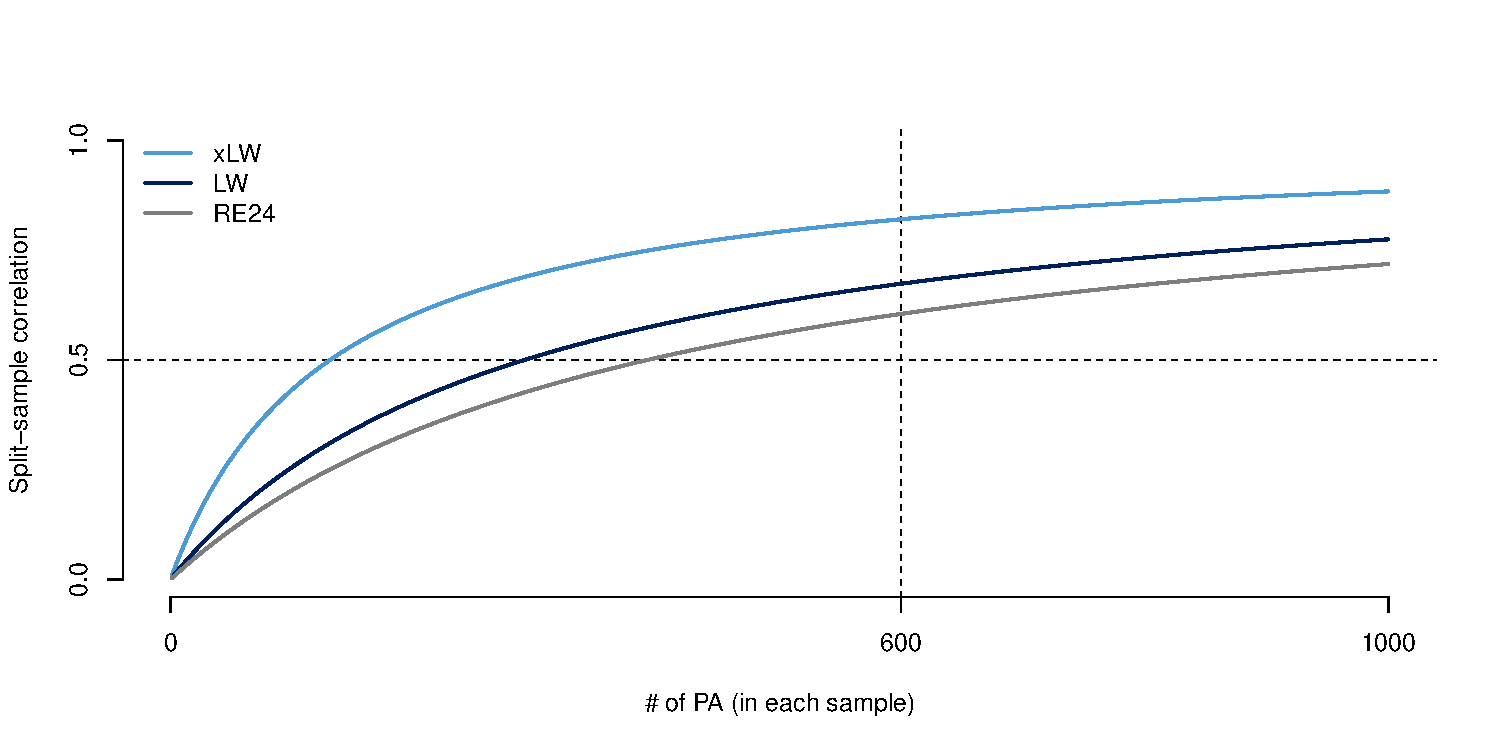
\includegraphics[width = \textwidth]{figures/re24_lw_xlw.pdf}
%\end{frame}

\begin{frame}{xLW vs. LW}
  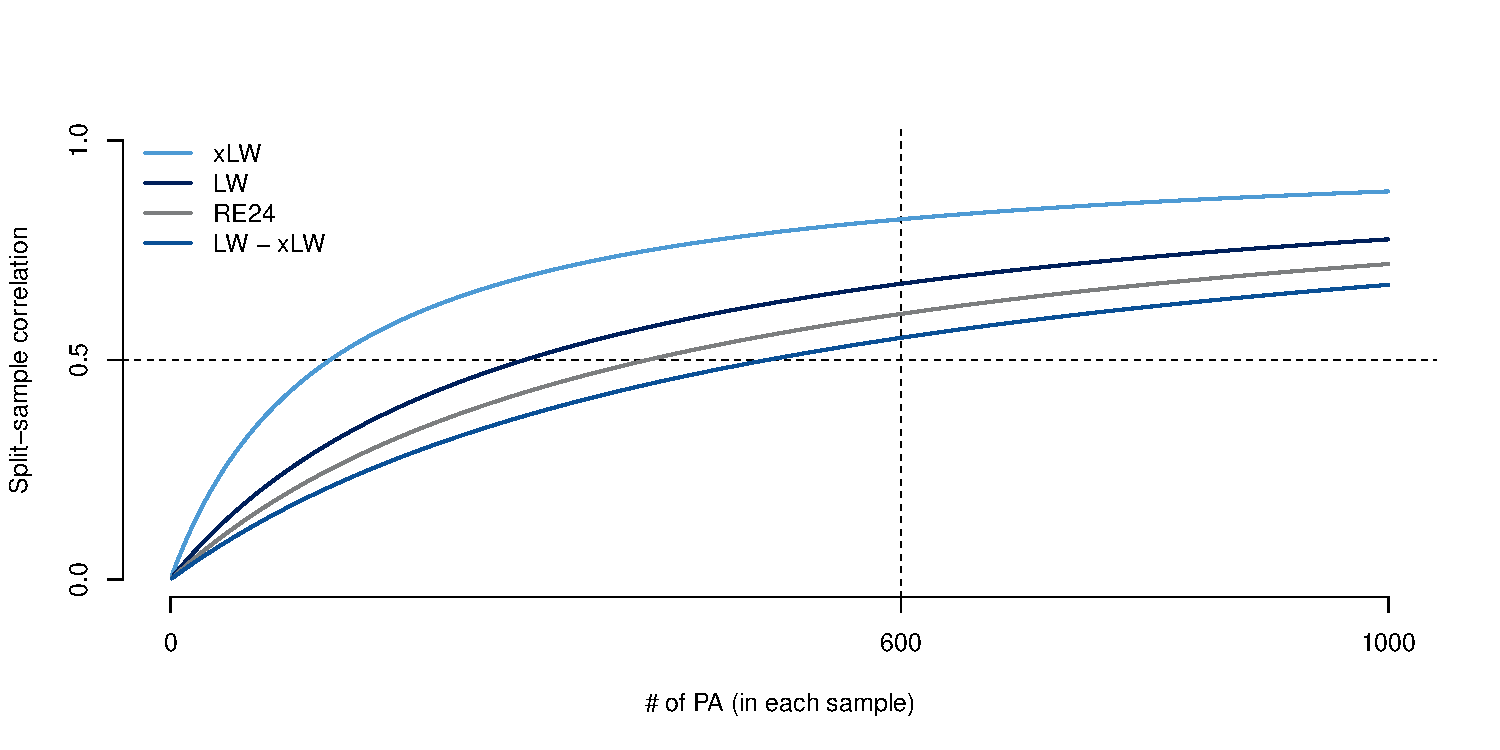
\includegraphics[width = \textwidth]{figures/re24_lw_xlw_diff.pdf}
\end{frame}

\begin{frame}{Takeaway \#2}
  Reliability is key in sport analytics, and the tradeoff between metrics depends on sample size. (Hint: You can blend them!)
\end{frame}

\begin{frame}
  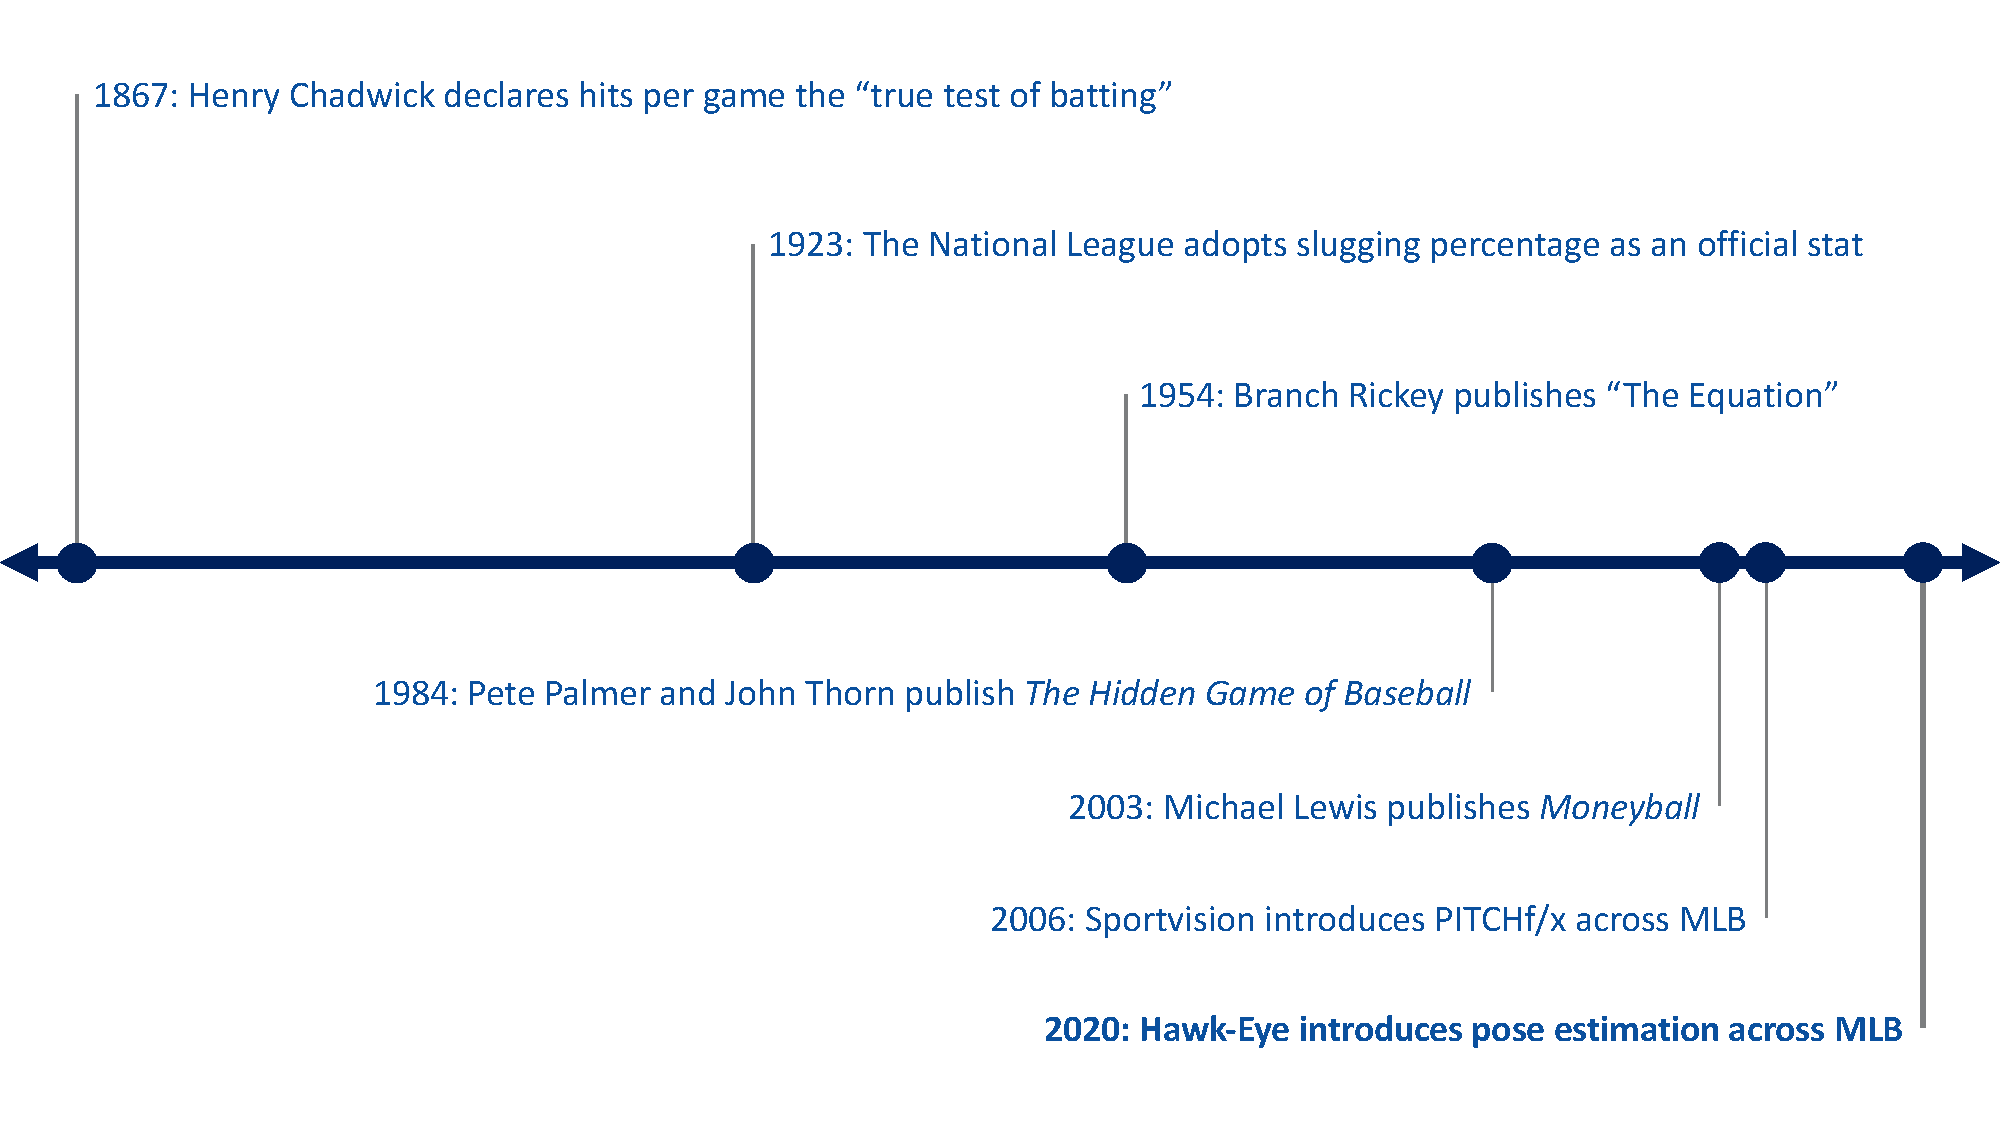
\includegraphics[width = \textwidth]{figures/timeline_2020.pdf}
\end{frame}

\begin{frame}{Hawk-Eye Camera System}
  \begin{columns}
    \begin{column}{0.6\textwidth}
      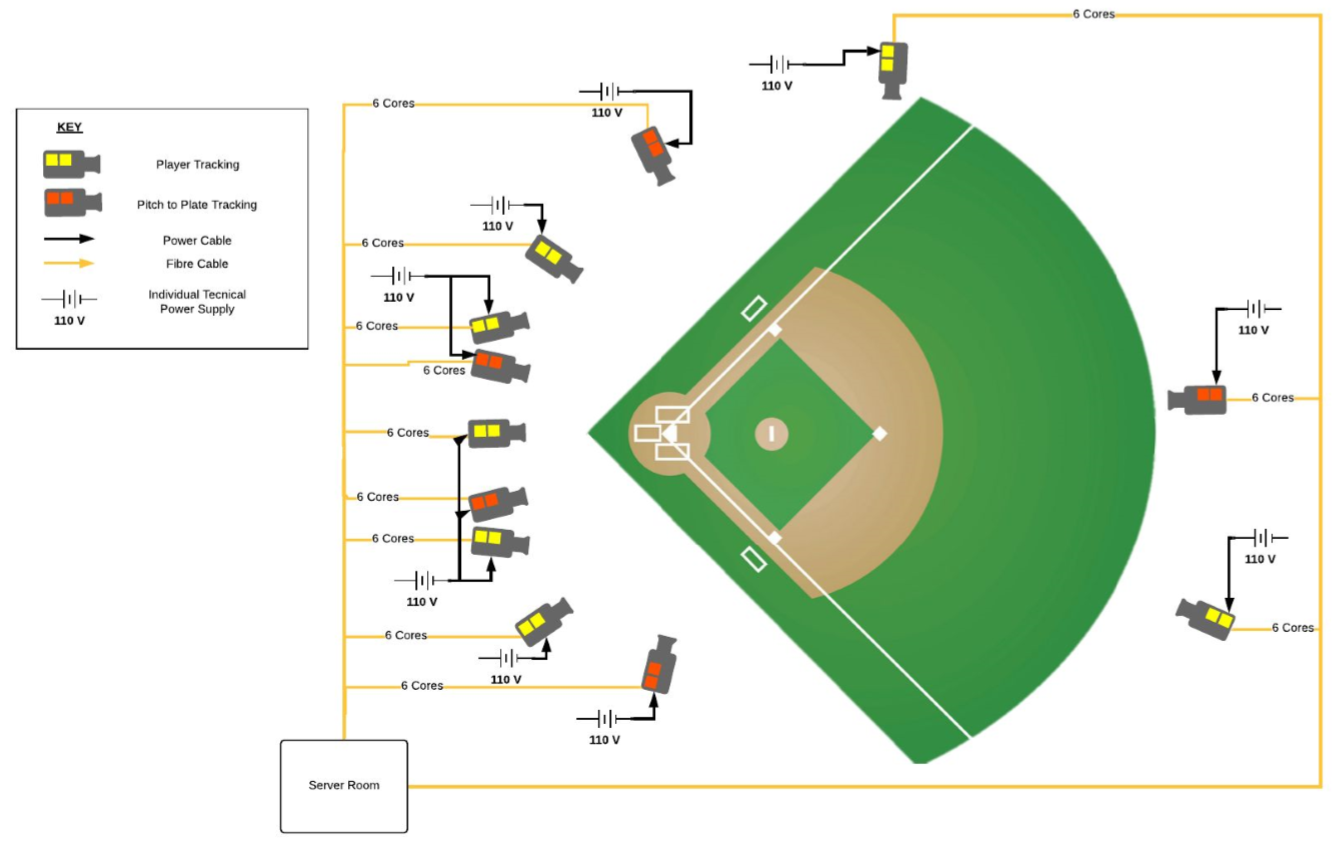
\includegraphics[width = \textwidth]{images/camera_system.png}
    \end{column}
    \begin{column}{0.4\textwidth}
      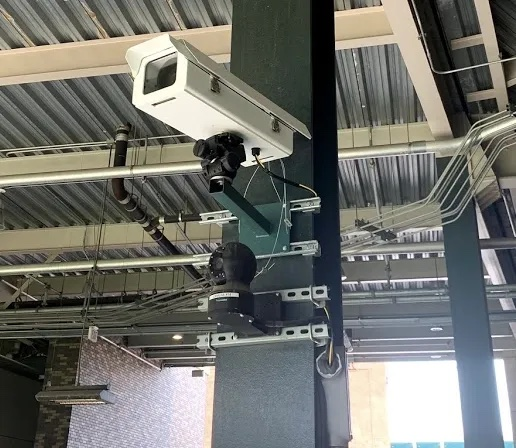
\includegraphics[width = \textwidth]{images/hawkeye_camera.jpeg}
    \end{column}
  \end{columns}
  \pause
  \begin{columns}
    \begin{column}{0.6\textwidth}
      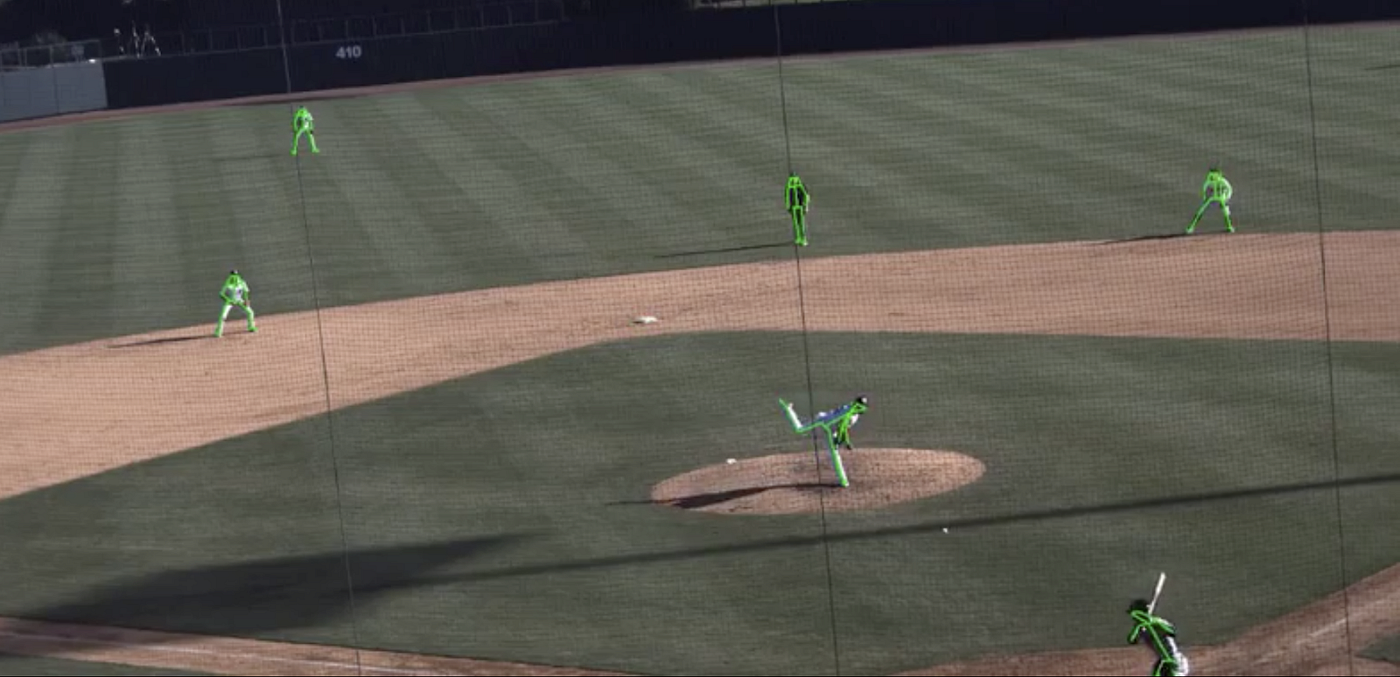
\includegraphics[width = \textwidth]{images/pose_tracking.png}
    \end{column}
    \pause
    \begin{column}{0.4\textwidth}
      \scriptsize
      \begin{itemize}
        \item 2020: Installed across MLB
        \item 12 cameras @ 50-100 fps
        \item Tracking \& pose estimation via computer vision
        \item Same tech used in tennis
        \pause
        \item 2023 $\rightarrow$ 300 fps!!
      \end{itemize}
    \end{column}
  \end{columns}
  \vfill
  \hfill\color{ricegray} \tiny Source: Ben Jedlovec (2020)\\
  \hfill https://technology.mlblogs.com/introducing-statcast-2020-hawk-eye-and-google-cloud-a5f5c20321b8
\end{frame}

\begin{frame}{Hawk-Eye Bat Tracking}
  \begin{columns}
    \begin{column}{0.6\textwidth}
      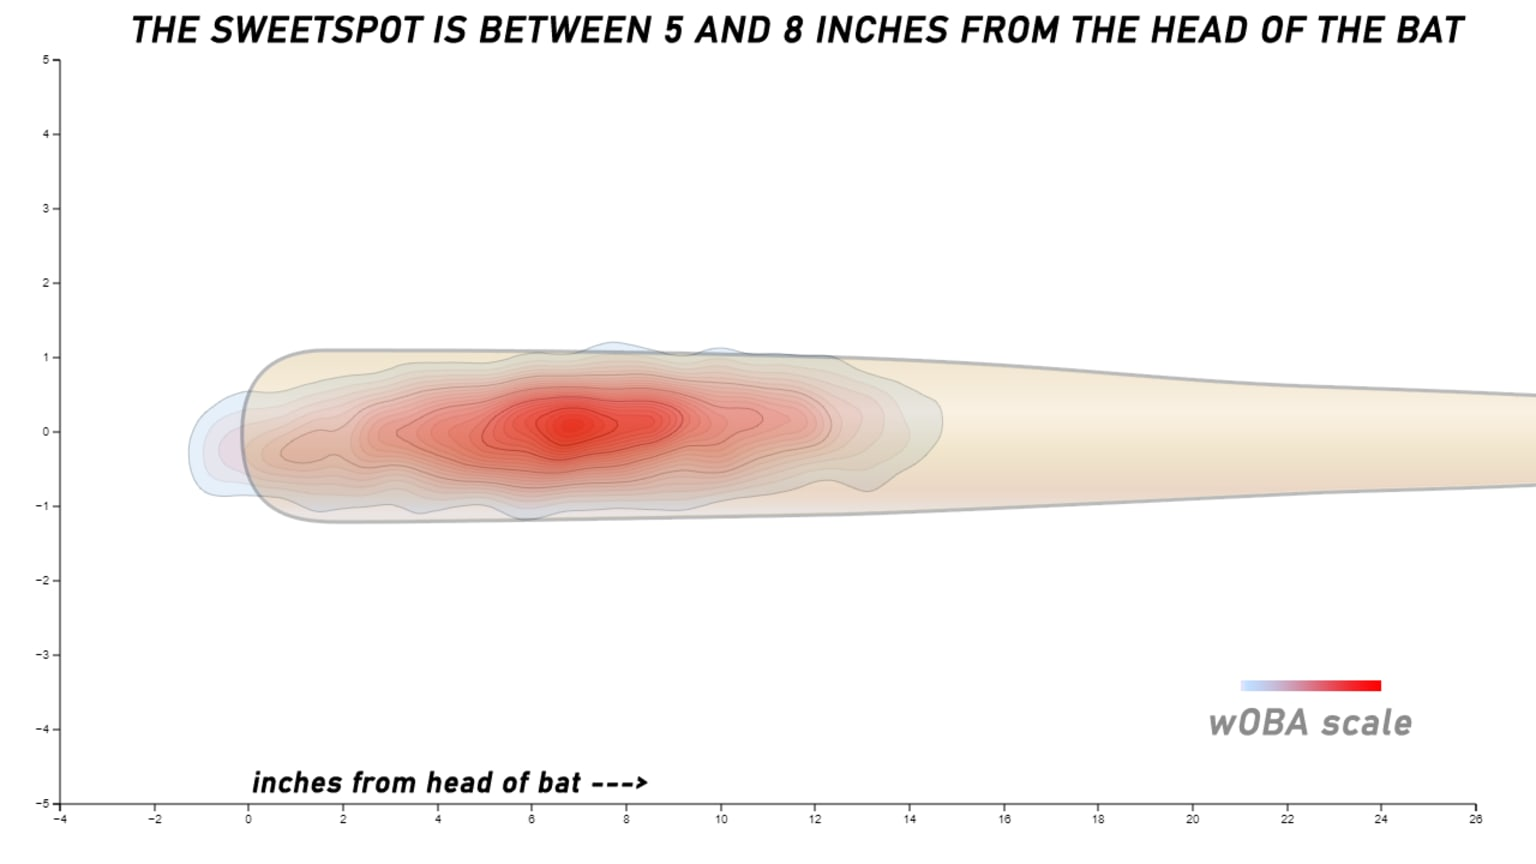
\includegraphics[width = \textwidth]{images/sweet_spot.jpg}\\
      \pause
      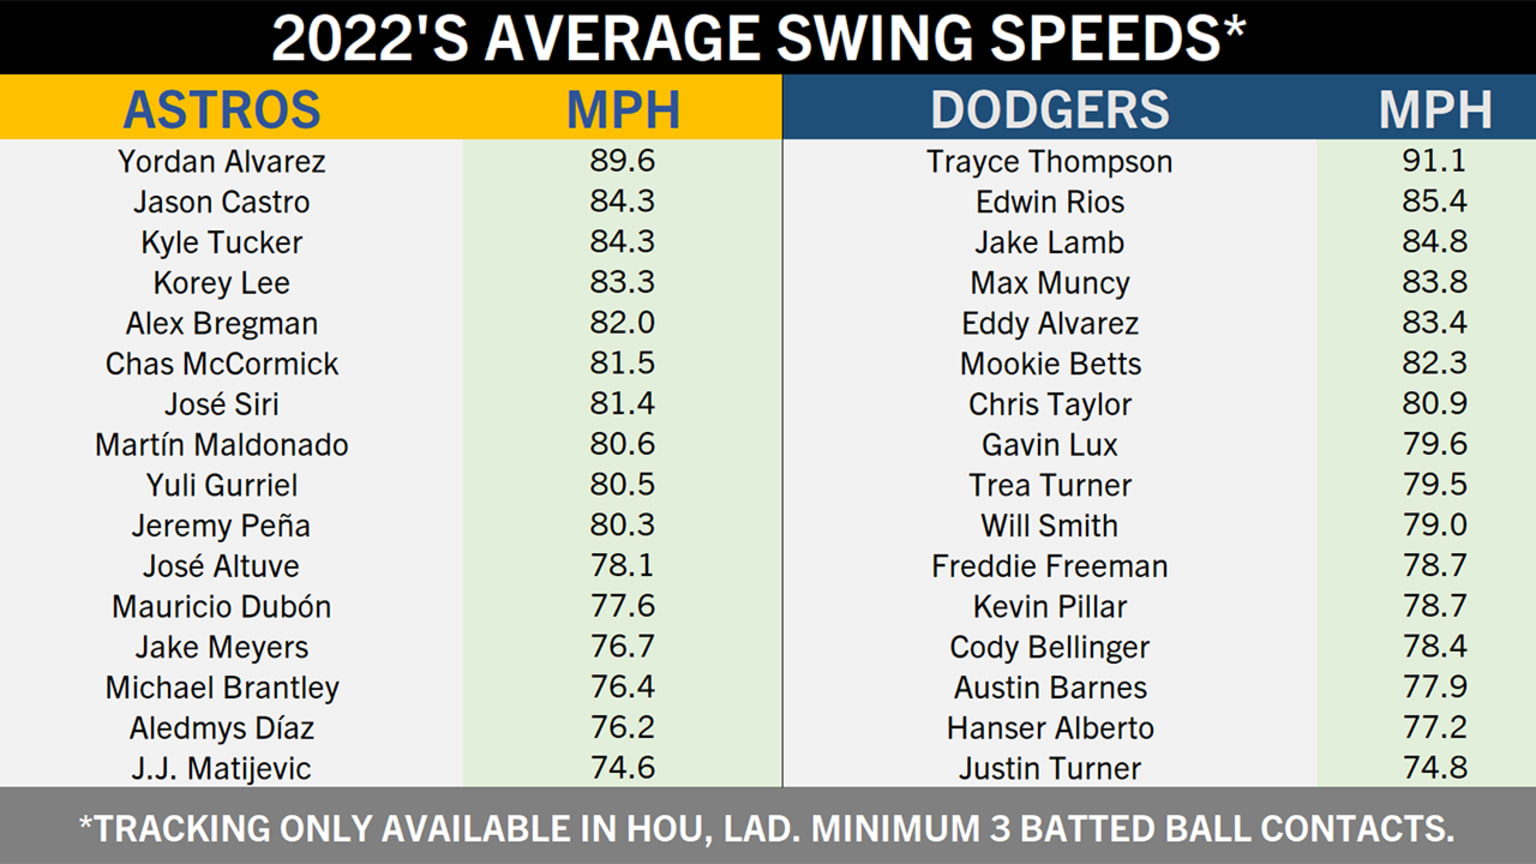
\includegraphics[width = \textwidth]{images/astros_dodgers.jpg}
    \end{column}
    \begin{column}{0.4\textwidth}
      \scriptsize \color{ricerichblue}
      \pause
      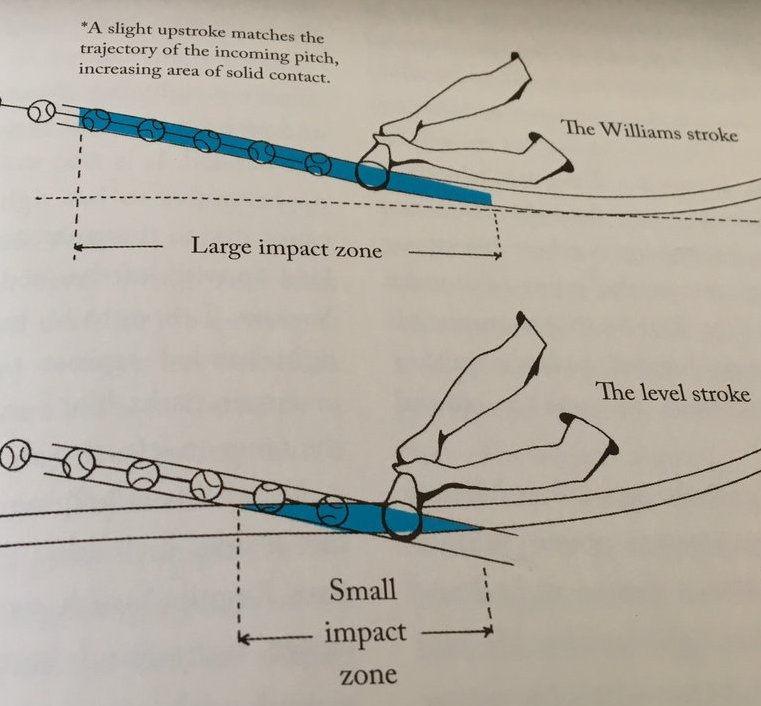
\includegraphics[width = \textwidth]{images/ted_williams.jpeg}\\
      Ted Williams\\
      {\it The Science of Hitting} (1970)\\
      c/o @JWonCATCHING
    \end{column}
  \end{columns}
  \vfill
  \hfill\color{ricegray}\tiny Source: Mike Petriello (2022)\\
  \hfill https://www.mlb.com/news/what-you-need-to-know-about-statcast-bat-tracking
\end{frame}

\begin{frame}{Takeaways}
  \begin{enumerate}
    \item Sport analytics is less {\it crafting} metrics and more {\it deriving} them.
    \item Reliability is key in sport analytics, and the tradeoff between metrics depends on sample size. (Hint: You can blend them!)
  \end{enumerate}
\end{frame}

\begin{frame}{Recommended Reading}
  \begin{columns}
    \begin{column}{0.5\textwidth}
      \centering
      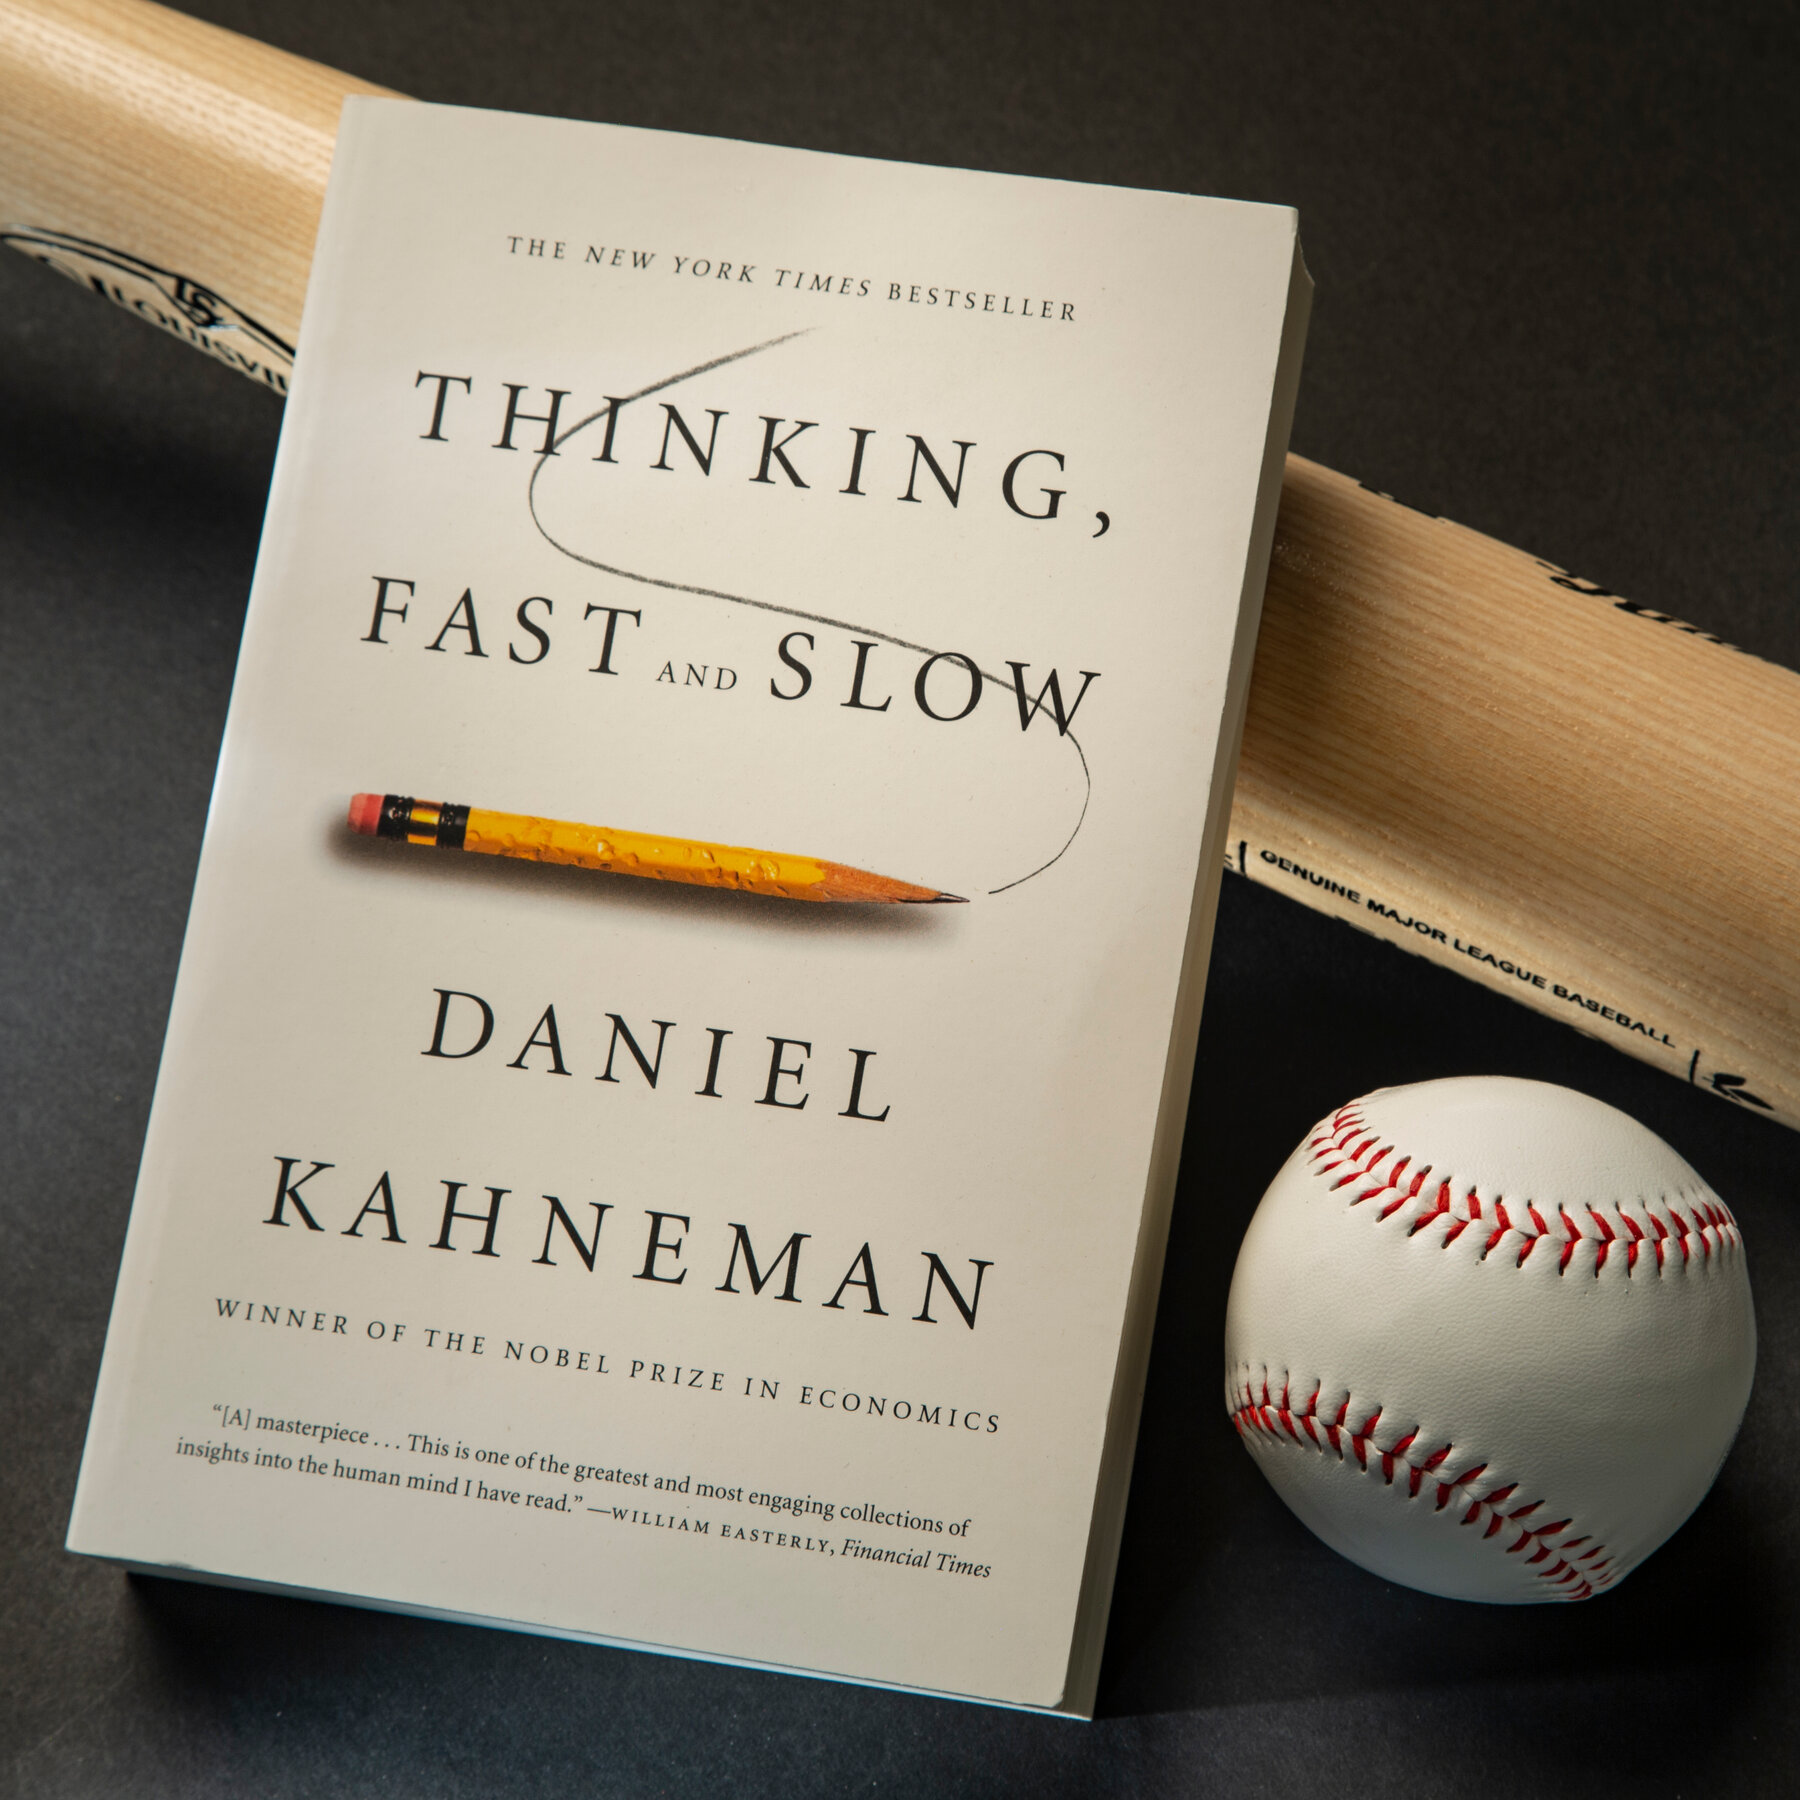
\includegraphics[height = 2in]{images/thinking_fast_and_slow.jpg}\\
      \color{ricegray} \tiny \it The New York Times
    \end{column}
    \begin{column}{0.5\textwidth}
      \centering
      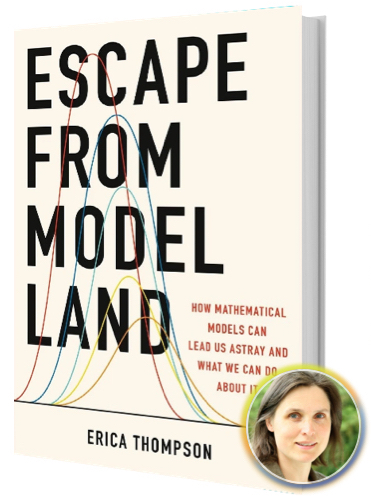
\includegraphics[height = 2in]{images/escape_from_model_land.jpg}
    \end{column}
  \end{columns}
\end{frame}

\begin{frame}
  \centering
  \LARGE
  Thank You!
\end{frame}

\end{document}
